\documentclass{article}

\usepackage{indentfirst}
\usepackage{graphicx}
\usepackage{setspace}
\usepackage{float}
\usepackage{hyperref}
\usepackage[margin=1in]{geometry}
\usepackage{booktabs}
\usepackage{csvsimple}
\usepackage{caption}
\usepackage{enumitem}
\usepackage{amssymb}
\usepackage{chngpage}
\usepackage[none]{hyphenat}

\hypersetup{colorlinks=true,linkcolor=blue,citecolor=blue}
\def\code#1{\texttt{#1}}

\usepackage[backend=biber, style=apa, sorting=nty]{biblatex}
\addbibresource{PhyloFisher.bib}

\title{PhyloFisher Manual}
\author{}
\date{June 2021}

\setcounter{secnumdepth}{0}


\begin{document}

\begin{titlepage}
    \begin{center}
         \begin{figure}[H]
        	   \centering
        	    	
\includegraphics[width=\linewidth]{figures/TREE-PF-LOGO.pdf}
            \end{figure}
        \textbf{v.1.0.12 Manual}\\
        PhyloFisher: A phylogenomic package for resolving eukaryotic relationships
        \vspace{0.2cm}
    \end{center}
        
        \textbf{Alexander K. Tice \textsuperscript{\ref{ins:msu_bio},\ref{ins:msu_igbb},*},
                David Žihala \textsuperscript{\ref{ins:ost_bio},*},
                Tomáš Pánek \textsuperscript{\ref{ins:msu_bio},\ref{ins:ost_bio},*},
                Robert E. Jones \textsuperscript{\ref{ins:msu_bio},\ref{ins:msu_igbb},\textasciicircum},
                Eric Salomaki \textsuperscript{\ref{ins:ceske_paras},\textasciicircum}, 
                Serafim Nenarokov \textsuperscript{\ref{ins:ceske_paras}}, 
                Fabien Burki \textsuperscript{\ref{ins:upp_bio},\ref{ins:upp_life}}, 
                Marek Eliáš \textsuperscript{\ref{ins:ost_bio}}, 
                Laura Eme \textsuperscript{\ref{ins:paris}}, 
                Andrew J. Roger \textsuperscript{\ref{ins:dalh}},
                Antonis Rokas \textsuperscript{\ref{ins:Van}}
                Xing-Xing Shen \textsuperscript{\ref{ins:China}}
                Jürgen Strassert \textsuperscript{\ref{ins:upp_bio},\ref{ins:Germ}}, 
                Martin Kolísko \textsuperscript{\ref{ins:ceske_paras},\ref{ins:ceske_bohe}\#}, 
                and 
                Matthew W. Brown \textsuperscript{\ref{ins:msu_bio},\ref{ins:msu_igbb},\#}}
        \vspace{0.15cm}
        
        \begin{enumerate}
            \itemsep0em
            \item Department of Biological Sciences, Mississippi State University, Mississippi State, MS, USA \label{ins:msu_bio}
            \item Institute for Genomics, Biocomputing \& Biotechnology, Mississippi State University, Mississippi State, MS, USA \label{ins:msu_igbb}
            \item Department of Biology and Ecology, Faculty of Science, University of Ostrava, Czech Republic \label{ins:ost_bio}
            \item Institute of Parasitology, Biology Centre Czech Academy of Sciences, České Budějovice,\\ Czech Republic \label{ins:ceske_paras}
            \item Department of Organismal Biology, Uppsala University, Norbyvägen, Uppsala, Sweden \label{ins:upp_bio}
            \item Science for Life Laboratory, Uppsala University, Norbyvägen, Uppsala, Sweden \label{ins:upp_life}
            \item Unité d’Ecologie, Systématique et Evolution, CNRS, Université Paris-Saclay France \label{ins:paris}
            \item Department of Biochemistry and Molecular Biology, Dalhousie University, Halifax, Nova Scotia,\\ Canada \label{ins:dalh}
            \item Department of Biological Sciences, Vanderbilt University, Nashville, TN, USA\label{ins:Van}
            \item State Key Laboratory of Rice Biology and Ministry of Agriculture Key Lab of Molecular Biology of Crop Pathogens and Insects, Institute of Insect Sciences, Zhejiang University, Hangzhou 310058, China \label{ins:China}
            \item Leibniz Institute of Freshwater Ecology and Inland Fisheries, Ecosystem Research, 12587 Berlin, Germany \label{ins:Germ}
            \item University of South Bohemia, Faculty of Science, České Budějovice, Czech Republic \label{ins:ceske_bohe}
        \end{enumerate}
        * and \textasciicircum \space Equally contributing author \\
        \# Corresponding authors


       \vfill
       
    \end{titlepage}
    \tableofcontents
    
    \pagebreak
    \section{Introduction}\label{sec:Intro}
        \subsection*{What is PhyloFisher?}
            PhyloFisher is a software package written in Python3 that can be used for the creation, analysis, and visualization of phylogenomic datasets that consist of protein sequences from eukaryotic organisms. Unlike many existing phylogenomic pipelines, PhyloFisher comes with a manually curated database of 240 protein coding genes from 304 eukaryotic taxa. However, the tool can be used to analyze any user-provided database. PhyloFisher is also equipped with a set of utilities to aid in running routine analyses performed during construction of or on constructed phylogenomic datasets and visualization of the results. If you use a component of PhyloFisher in your research, please cite:\\
            
            Tice et al. (2021). PhyloFisher: A phylogenomic package for resolving eukaryotic relationships. doi. xxxxxxx. 
        
        \subsection{Compatible Operating Systems}
            \begin{description}
                \itemsep0em
                    \item Linux
                    \item macOS
                    \item Windows (forest.py \& ParaSorter ONLY!)
            \end{description}

        
        \subsection{Space Requirements}
            Allow \textasciitilde4GBs for installation including provided database. \textasciitilde2GBs software only. % ~ not present in document
        
        \subsection{Third Party Software Utilized by PhyloFisher}
            \begin{description}
                \itemsep0em
                
                \item ASTRAL-III v. 5.7.3 (\cite{zhang_astral-iii_2018}) 
                \item BLAST v. 2.9.0 (\cite{Altschul1990})
                \item BMGE v. 1.1.2 (\cite{criscuolo_bmge_2010})
                \item CD-HIT v. 4.8.1 (\cite{fu_cd-hit_2012})
                \item DIAMOND v. 09.24 (\cite{buchfink_fast_2015})
                \item dist\_est v.1.0 (\cite{susko_estimation_2003})
                \item Divver v. 1.01 (\cite{ali_identifying_2019})
                \item ETE3 3.1.1 (\cite{Huerta-Cepas})
                \item FastTree v. 2.1.11 \cite{price_fasttree_2010}
                \item HMMER v. 3.2.1 (\cite{mistry_challenges_2013})
                \item MAFFT v.7.455 (\cite{katoh_mafft_2013})
                \item MAMMaL v.1.1.1 (\cite{susko_accelerated_2018})
                \item OrthoMCL v 5.0 (\cite{chen_orthomcl-db_2006})
                \item PREQUAL v. 1.02 (\cite{whelan_prequal_2018})
                \item RAxML v. 8.2.12 (\cite{stamatakis_raxml_2014})
                \item trimAl v.1.4.rev15 (\cite{capella-gutierrez_trimal_2009})
            \end{description}
    \pagebreak
    
        \subsection{PhyloFisher Package Contents}
        \begin{itemize}
            \item Manually curated database of 240 orthologs and their paralogs from 304 eukaryotic taxa. These taxa cover the known diversity of eukaryotes.
            \item Main Workflow tools for:
                \begin{itemize}
                    \item The preparation of custom databases composed of protein coding genes in lieu of the provided database
                    \item Ortholog and paralog “mining” from input proteomes
                    \item Evaluating completeness in the database of newly input data
                    \item Automated removal of non-homologous sites, alignment, trimming, length filtering and single gene tree construction
                    \item Visualization of single gene trees and interactive selection of orthologs, paralogs, and removal of contamination
                    \item Generation of final statistics post ortholog selection and contamination removal
                        \begin{itemize}
                            \item Can be subset by user provided thresholds of completeness or by assigned taxonomy.
                        \end{itemize}
                    \item Creation of chimeric taxa for use in phylogenomic analyses
                    \item Automated concatenation of phylogenomic matrices
                \end{itemize}
            \item Utilities for:
                \begin{itemize}
                    \item Alternative genetic code prediction
                    \item Compositional bias testing (amino acid re-coding)
                    \item The removal of fast evolving sites from a phylogenomic dataset
                    \item The removal of fast evolving taxa from a phylogenomic dataset
                    \item Detection and removal of the most heterotachious sites in a phylogenomic dataset
                    \item Examining the number of occurrences of clades  of interest in bootstrap trees
                    \item Matrix construction from randomly re-sampled genes from a phylogenomic dataset
                    \item Binning single-protein trees based on Relative Tree Certainty (RTC)
                    \item collapsing of multiple proteomes to produce a single “most complete” proteome with regards to the database (useful for  single-cell data and to form chimeric taxa from closely related species)
                \end{itemize}
        \end{itemize}

        \begin{figure}[H]
            \centering
        	 \includegraphics[width=\linewidth]{figures/Figure1_general_workflow-EDITED5.pdf}
        	  \caption{Overview of the PhyloFisher workflow and package contents. The PhyloFisher package consists of a manually curated database of 240 protein coding genes and their paralogs from 304 eukaryotic taxa; a series tools to perform the essential steps of phylogenomic dataset construction (homolog collection, single-protein tree construction, removal of paralogs and contaminants, matrix concatenation); and many pre and post-construction analyses necessary for a publication-quality phylogenomic study.}
        	  \label{Fig:workflow}
        \end{figure}
        
        \subsection{Terminology Used Throughout the PhyloFisher Manual}
            Throughout this manual different collections/types of data are referred to using specific names in an attempt to provide clarity to the exact set of data being referenced (\autoref{Fig:terminology}). \\\\
            The seven collections of data referenced in the manual are:
            \begin{enumerate}
                \item \textbf{Database} - the database is a collection of manually curated sequences demarcated as either orthologs or paralogs. This can refer to either the provided database or a custom database supplied by the user. Final decisions regarding orthology and paralogy made by a user during manual curation of sequences collected from newly input proteomes are stored here. The initial database provided has been manually curated prior to its release, however the application of different phylogenetic methods, manual curation practices, and taxon selection will cause the user's database to change over time.
                \item \textbf{Working Dataset} - the purpose of the working dataset is to aid in the identification of orthologs, paralogs, and contaminants from input proteomes.  The working dataset is created when sequences are collected by fisher.py from input proteomes and appended to the copies of the corresponding homolog files from the database. These data will then move through the PhyloFisher workflow until final decisions based on manual curation have been applied to the database. A working dataset is not revisited after decisions from manual curation have been made and applied to the database.
                \item \textbf{Phylogenomic Dataset} - A set of orthologs and taxa in the form of individual ortholog alignments and a concatenated matrix of these alignments that have been selected from the database to perform phylogenomic analyses on. 
        \begin{figure}[H]
            \centering
        	 \includegraphics[width=\linewidth]{figures/Dataset_explanation_fig.pdf}
        	 \caption{Flow chart of the PhyloFisher workflow documenting how collections of data are referenced throughout the manual.}
        	 \label{Fig:terminology}
        \end{figure}
                \item \textbf{Gene(s)} - The term gene is used throughout this manual to refer to a group of closely related homologs (similar to a gene family). These genes are named based on the corresponding human or \textit{Arabidopsis thaliana} orthologs that were used as queries in BLAST searches to collect sequences from other eukaryotic organisms during the construction of the phylogenomic database developed in \cite{tice_expansion_2016}. The aforementioned database was used as a starting point for construction of the PhyloFisher v1.0 database. We have chosen not to use either of the terms “gene family” or “orthogroup” because these genes only contain the most similar sequences to the initial search query rather than all potential members.
                \item \textbf{Ortholog(s)} - The term ortholog, in the context of PhyloFisher, refers to a sequence(s) within the database that will ultimately be used for the construction of phylogenomic datasets. Additionally, the term ortholog is applied to the putative sequence from each newly added taxon that was selected by the fisher.py algorithm for use in phylogenomic datasets, pending decisions made during manual curation.
                \item \textbf{Paralog(s)} - The term paralog, in the context of PhyloFisher, refers to sequences that are included in working datasets to enable proper ortholog selection and to reveal frequency of duplications in a particular gene and taxonomic group. The databases paralogs help users  avoid the inclusion of sequences from different paralogs for different species and thus avoid the generating incorrect phylogenetic signal in the final dataset. Sequences denoted paralogs after each round of manual curation are not to be used in the construction of phylogenomic datasets. Additionally, the term paralog refers to sequences that are collected from newly input taxa that were not selected by the fisher.py algorithm as the putative ortholog, pending decisions made during manual curation. They can also represent hidden contaminants or variants of the same contig (e.g. due to a retained intron(s)). After manual curation all sequences that are denoted as “paralogs” will be stored in the database to be utilized during manual curation of subsequent taxon additions.
                \item \textbf{Homolog(s)} - The term homolog is used when referring to datasets that consist of both orthologs and paralogs (such as the working dataset), or to describe the relationship between orthologs and paralogs. 
            \end{enumerate}
            
        \subsection{PhyloFisher's Provided Database}
        
            \subsubsection{PhyloFisher's Provided Database Is...}
                The PhyloFisher package is equipped with a manually curated database of 240 protein coding genes from up to 304 eukaryotes that can be used for phylogenomic analyses of eukaryotic organisms. Details on the genes and taxa included in the database can be found currently at the below link.  A metadata file (metadata.tsv) that provides information on the proteomes used in database construction is included with the database and can be found in the directory database/. In addition to a single ortholog of each of the databases’s 240 genes, a database of each gene's paralogs is maintained.
                
            \subsubsection{PhyloFisher's Provided Database Is Not...}
                A set of genes that are universally present and single copy in all eukaryotic taxa included in the database.
                
        \subsubsection{How a User’s PhyloFisher Database Changes Over Time}
        Regardless of whether a user chooses to utilize the provided database or their own custom database, the nature of the PhyloFisher workflow changes the chosen database overtime in a way that increases the database’s ability to inform a user on levels and phylogenetic location of paralogy for each gene in the database. Typically, the addition of new taxa to phylogenomic databases, especially underrepresented lineages, often reveals previously unknown or “hidden” paralogy. This previously unknown paralogy can exist at any level from shallow and species specific to ancient paralogy that simply could not be inferred with the previous database. Depending on the level of paralogy and the user’s phylogenetic question, accidental inclusion could have dramatic effects on phylogenomic inference and subsequent interpretations of evolutionary events based on the resulting phylogenomic tree. Once revealed, newly discovered paralogs are demarcated as such and maintained in the paralog portion of the database to aid in the identification of the paralog from newly added taxa in subsequent rounds of addition and prevent inclusion in future phylogenomic datasets. By continuously keeping a record of all known paralogs regardless of their emergence in evolutionary time a user’s decision regarding ortholog selection will always be the most informed even if/when the depth of their phylogenetic questions change over time. Our strategy also allows for the construction of a larger/more complete phylogenomic dataset as the most well represented orthologs can be chosen for phylogenomic analyses. 
                
         Users do have the option of slimming down the database through complete deletion of taxa. User’s may also choose to exclude an organism and/or the organism’s paralogs from the working dataset used for single gene tree construction. While these options are provided to ease the computational burden of single gene tree construction, we highly recommend using as many taxa and their associated paralogs as feasible. Experience has shown that including more taxa will lead to more informed ortholog selection and therefore a more reliable final tree.
                
        \subsection{Ortholog Selection via the Fisher Algorithm}
            Ortholog selection and paralog demarcation is performed using the python script fisher.py (\autoref{Fig:algorithm}) that requires two inputs: predicted proteome(s) to be added to the database and an input-metadata file containing key information about them. To remove redundancy in the input proteome (typical when proteomes are predicted in silico from transcriptomic data), fisher.py invokes CD-HIT v.4.8.1 (\cite{fu_cd-hit_2012}) with the option “-c 0.98”, which clusters sequences globally at a similarity threshold of 98\%. Next, hmmsearch from the software package HMMER v. 3.2.1 (\cite{mistry_challenges_2013}) is run on the input proteome using a pre-computed profile Hidden Markov Model (HMM) of each protein alignment in the database. Up to a user-defined number of sequences are collected (default = 5) that meet the significance threshold (e-value < 1e -10). If no sequence meets the significance threshold, the script moves on to the next protein. If sequences are found (up to the user-defined number), they are prioritized based on the level of significance (i.e., the sequence with the most significant hit is preliminarily denoted as the most likely putative ortholog with other included sequences preliminarily denoted as putative paralogs). From here, the algorithm proceeds in either of two directions, depending on information given in the input metadata file. In the two routes outlined below, sequences can be added to or removed from the initial sequences collected by hmmsearch, as they meet or fail to meet the outlined criteria. The prioritization of a sequence can also change within the list based on the criteria outlined below. At the end of either route, if only one sequence remains, it is considered the putative ortholog for the input taxon. If more than one remains, the sequence with the highest priority in the list is considered the putative ortholog and the other retained sequences are considered putative paralogs. All retained are added to the corresponding single-protein alignment.
            
            \subsubsection{Default Route}
                If no related species present in the database is/are listed in the “Blast Seed” column of the input metadata file to use as specific queries, each sequence collected from the initial hmmsearch is used as the query in a search using DIAMOND v. 09.24 (\cite{buchfink_fast_2015}) against OrthoMCL v 5.0 (\cite{chen_orthomcl-db_2006}) with the options “blastp -e 1e-10 --more-sensitive.” Any sequence that has a significant hit (e-value < 1e -10) to a bacterial orthogroup in OrthoMCL is discarded along with any sequence that does not have a significant hit to the OrthoMCL orthogroup corresponding to the respective profile HMM used to retrieve the sequence. Retained sequences are again used as queries in a DIAMOND search using the parameters given above against the database. Query sequences whose best hit represents the conserved gene corresponding to the initial profile HMM that retrieved the query sequence is retained and added to the alignment. The remaining sequence that has the highest priority based on the initial hmmsearch is considered to be the putative ortholog and any other surviving sequences are labelled putative paralogs.
                
            \subsubsection{Phylogenetically Informed Route}
                The input metadata file gives users the option to specify taxa already in the database whose sequences will be used as queries for blast searches against the new organism’s proteome; typically these should be closely related to the newly added taxon. Any number of species already present in the database may be chosen to serve as specific queries, but the algorithm will use them in the order provided, and, in cases outlined below, may not proceed to subsequent taxa. If species to be used as specific queries are listed in the input metadata file, fisher.py will initially pick the sequence representing a particular orthologous gene group (“ortholog” for simplicity) from the first organism listed, if present. If absent in the database, fisher.py will sequentially check for the ortholog from the remaining taxa listed. If the orthologs from one or more of the subsequent taxa are found, the algorithm proceeds as outlined below. If no ortholog from all listed organisms can be found, fisher.py will proceed to the default route for this particular protein. If an ortholog is present in at least one of the listed species, then its sequence is used as the query in a BLAST (Camacho et al. 2009) search against the input organism’s predicted proteome. If no significant hit (e-value < 1e -10) is found, fisher.py will use the ortholog of the next listed species, if one is provided. If no other species is listed, the ortholog is not present in the database for the listed species, or if the orthologs of all listed species do not return a significant BLAST hit, the protein is skipped for the input taxon. If significant BLAST hits are found, up to a user-defined number of those (default = 5) are collected and examined further. The sequences from the original hmmsearch are reprioritized based on the level of significance of the BLAST hit. The sequence with the most significant hit becomes the priority sequence, unless it was not also collected by the initial hmmsearch: any sequence that produces a significant BLAST hit but was not collected in the initial hmmsearch is discarded. The retained sequences are then used as queries against OrthoMCL. Any sequence that has a significant hit (e-value < 1e -10) to a bacterial orthogroup in OrthoMCL is discarded along with any sequence that does not have a significant hit to the OrthoMCL orthogroup corresponding to the respective profile HMM used to retrieve the sequence. Next, all the sequences that have passed the filtering in the previous step are compared with blast against the database of conserved marker proteins. If the query sequence’s best blast hit is a sequence corresponding to the profile HMM that retrieved the query sequence in the initial search, the sequence is retained. If the sequence’s best blast hit is a sequence from another alignment, the sequence is still retained, but is written out to the file “non\_corresponding\_hits.txt” with a note on which protein from the database represents the best blast hit. Sequences are then added to the corresponding dataset from the database and aligned using MAFFT v.7.455 (\cite{katoh_mafft_2013}) with the parameters “--auto --reorder”, trimmed with trimAl v.1.4.rev15 (Capella-Gutiérrez et al. 2009) with a gap threshold of 0.2, and subjected to phylogenetic tree reconstruction via FastTree v. 2.1.11 (\cite{price_fasttree_2010}) with default parameters. The resulting tree is examined using the python package ETE3 (\cite{Huerta-Cepas}). By default sequences that branch sister to or within a clade composed of organisms with the same assigned higher taxonomy are retained while sequences that branch outside of the assigned higher taxonomy are eliminated unless no sequence branches with sequences assigned the correct higher taxonomy. This happens regardless of previous criteria. Higher taxonomy for taxa is derived either from the database’s metadata file or the input metadata file. Finally, a length filtration step will remove any sequences that have more than 70\% gaps in the trimmed alignment. All retained sequences are then added to their corresponding alignments from the database, with the sequence that received the highest level of priority being denoted the putative ortholog and all others denoted as putative paralogs.
        \begin{figure}[H]
            \centering
        	 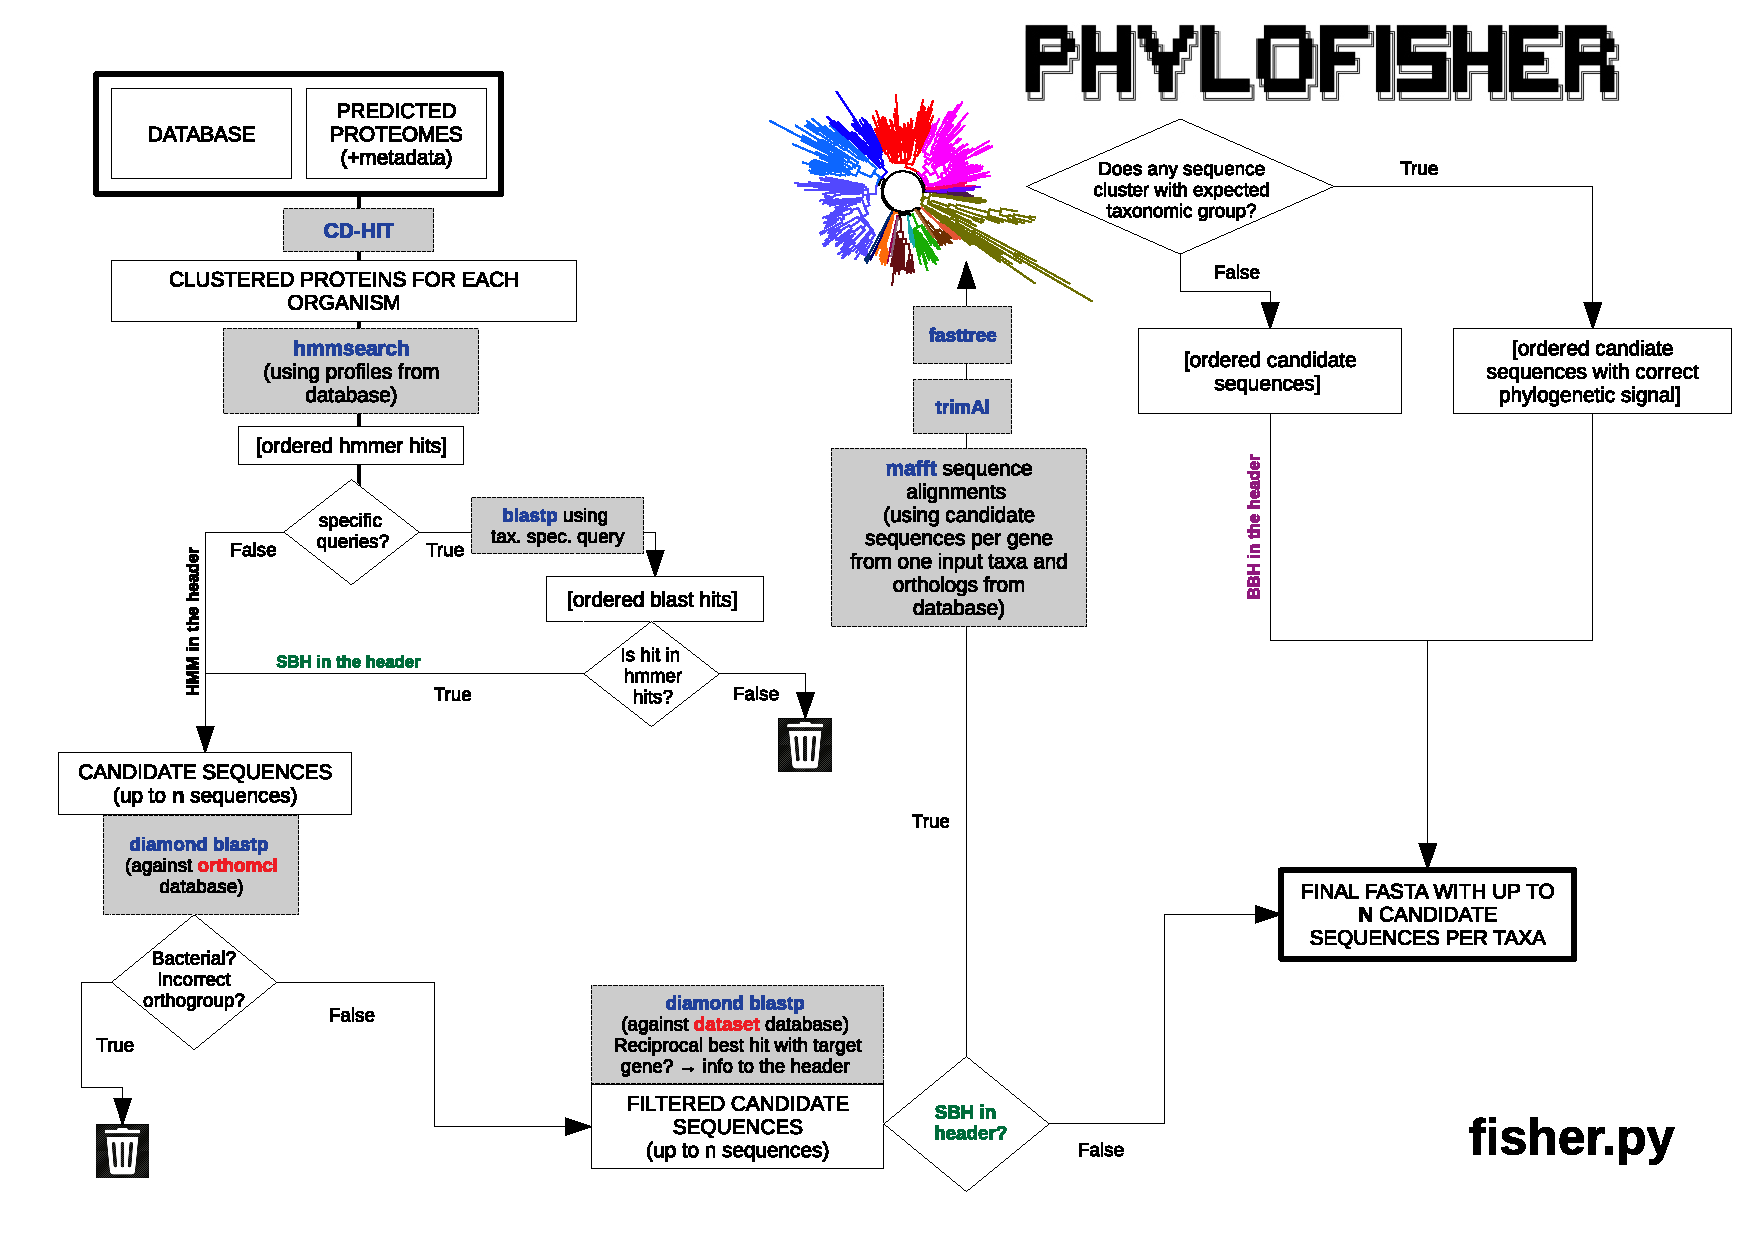
\includegraphics[width=\linewidth]{figures/Figure2_fisher_algorithm.pdf}
        	 \caption{Flowchart of homolog collection performed by the PhyloFisher python script fisher.py. Briefly, each predicted proteome of a new taxon to be added is processed through either a default route, or a phylogenetically aware route that utilizes the manually curated orthologs from closely related taxa chosen by the user (and present in the database) as search queries against the proteome of the new taxon. Up to a user-defined number of collected sequences are reprioritized or eliminated based on a set of criteria designed to maximize correct demarcation of the desired ortholog and related paralogs while avoiding contaminating sequences. See section “Ortholog Selection via the Fisher Algorithm” of this guide for a detailed description of the logic, third-party software and associated parameters utilized.}
        	 \label{Fig:algorithm}
        \end{figure}
        
        \subsection{Automated Filtering, Alignment, Trimming, and Single Gene Tree Construction}
        \label{sec:sgtmethods}
            PhyloFisher also includes a python script sgt\_constructor.py to automatically filter, align, trim, length filter, and construct phylogenetic trees from all homolog alignments. The script takes the output files from fisher.py (original single-protein alignments that now contain newly added sequences selected by the fisher algorithm for input taxa as well as the previously denoted paralogs from the database) and removes any dashes to produce an unaligned set of sequences for non-homologous character removal via PREQUAL v. 1.02 (\cite{whelan_prequal_2018}) using the default settings. Next, a length filtering step is performed to minimize the inclusion of proteins predicted from fragments of the same gene. This is common in proteomes predicted from transcriptomes. First, sequences are aligned with the program MAFFT using the settings “--globalpair --maxiterate 1000 --unalignlevel 0.6”. This is followed by assessment of alignment error and uncertainty by the program Divvier v. 1.01 (\cite{ali_identifying_2019}) using the options “-partial -mincol 4 -divvygap”. The resulting alignments are trimmed using BMGE v. 1.1.2 (\cite{criscuolo_bmge_2010}) with a gap-rate cutoff of 0.3. Any sequence whose length is less than half the total alignment length, after BMGE filtering, is removed. After removal of “short” sequences, files are prepared for single-protein phylogenetic tree construction by rerunning MAFFT and Divver as above, followed by trimming with the program trimAl with a gap threshold of 0.01. Finally, single-protein tree reconstruction is performed using RAxML v. 8.2.12 (\cite{stamatakis_raxml_2014}) with the options “-m PROTGAMMALG4XF -f a -x 123 -N 100 -p 12345”. When single gene tree construction begins “sgt\_constructor.py” will check to see how many gene trees are to be built and how many threads were provided by the user. If the number of gene trees to be built is greater than the number of threads provided, “sgt\_constructor.py” will run as many jobs as it can using a single thread each. This process will continue until all gene trees have been built. If the total number of gene trees to be built is less than the number of threads available “sgt\_constructor.py” will distribute all threads available as evenly as possible.
            
    \section{Getting Started with PhyloFisher}

        PhyloFisher can be installed and updated via Conda or PIP.
        \subsection{Installation via Anaconda}
        \begin{enumerate}[itemsep=12pt]
            \item If you do not already have conda installed, please install via \href{https://docs.conda.io/projects/conda/en/latest/user-guide/install/}{Anaconda}.
                
            NOTE: Installation via Miniconda will complete. However, all non-python dependencies will not be installed. In short, installation via Miniconda will NOT work.
            
            \item Install mamba via conda
            \\\\
            \code{conda install mamba}
            \item Prepare a conda virtual environment via mamba \label{step:env}:
            \\\\
            \code{mamba create -n fisher}
            \item Activate the environment you just created:
            \\\\
            \code{conda activate fisher}
            \item Add the following Anaconda Cloud channels to your channels:
            \\\\
            \code{conda config --append channels phylofisher}
            
	        \code{conda config --append channels bioconda}
	        
	        \code{conda config --append channels conda-forge}
            \item Now install PhyloFisher:
            \\\\
            \code{mamba install phylofisher}
            \\\\
            NOTE: when conda virtual environment is active all PhyloFisher python scripts are now in your path and you can access them by typing the first few letters and tab.
        \end{enumerate}
        
        \subsection{Installation via PIP}
        \begin{enumerate}
            \item Install PhyloFisher via PIP
            \\\\
           \code{pip install phylofisher}
            \item Install non-python dependencies
            \\\\
            linux: \code{install\_deps.py}
        
            macOS: \code{install\_deps.py --gxx </path/to/g++/executable>}
            \\\\
            NOTE: The gcc compiler is required for installing non-python dependencies on macOS. If you do not already have the gcc compiler it can be quickly installed via brew by running:
            \\\\
            \code{brew install gcc}
            \\\\
            NOTE: After PIP installation, all PhyloFisher python scripts are now in your path and you can access them by typing the first few letters and tab.
        \end{enumerate}
        
        \subsection{Installation of forest.py \& ParaSorter locally (including Windows)}
        Installation of these two tools on a users local machine is required for downstream steps in the PhyloFisher workflow. Although the entire PhyloFisher software package does not run on Windows, this minimal download will. This download will provide users (including Windows users) the graphical tree parsing aspects of the package on their local machines. This minimal download of forest.py and ParaSorter can be retrieved from the "ParaSorter" section of  \href{https://github.com/TheBrownLab/PhyloFisher/tree/master/parasorter}{PhyloFisher GitHub Repository}. 
        \\\\
        Further documentation on the usage of both forest.py and Parasorter can be found in steps 9 and 10 in the "Detailed Example Workflow" section of this manual respectively.
        
        \subsection{Download PhyloFisher’s Provided Database or Prepare a Custom Database.}
        \subsubsection{Download PhyloFisher’s Provided Database}
        \begin{enumerate}
            \item Retrieve the provided starting database via wget:
            \\\\
            \code{wget https://ndownloader.figshare.com/files/29093409}
            \item Uncompress the .tar.gz file:
            \\\\
            \code{tar -xzvf 29093409}
        \end{enumerate}
        The uncompressed database directory contains the subdirectories and files detailed below.
        \begin{itemize}
            \item database/
                \begin{itemize}
                    \item backups/
                        \begin{itemize}
                            \item \{Month\}\_\{Day\}\_\{Year\}.tar.gz (a compressed file containing backups of the two database folders orthologs/, paralogs/, the database file metadata.tsv, and tree\_colors.tsv
                        \end{itemize}
                    \item datasetdb/
                        \begin{itemize}
                            \item datasetdb.dmnd (a diamond database of the PhyloFisher v 1.0 orthologs)
                            \item datasetdb.fasta (a fasta file of the PhyloFisher v 1.0 orthologs used to construct the diamond database
                        \end{itemize}
                    \item orthologs/
                        \begin{itemize}
                            \item \{gene\_name\}.fas (240 fasta files of the PhyloFisher v 1.0 orthologs )
                        \end{itemize}
                    \item orthomcl/
                        \begin{itemize}
                            \item bacterial (abbreviated names of bacterial species present in OrthoMCL v. 5.0)
                            \item gene\_og (a tsv file detailing the names of the 240 PhyloFisher v 1.0 genes and their corresponding  OrthoMCL v. 5.0 orthogroup number(s))
                            \item orthomcl.diamonddb.dmnd (diamond database of OrthoMCL v. 5.0)
                        \end{itemize}
                    \item paralogs/
                        \begin{itemize}
                            \item \{gene\_name\}\_paralogs.fas (240 fasta files of the PhyloFisher v 1.0 paralogs)
                        \end{itemize}
                    \item profiles
                        \begin{itemize}
                            \item \{gene\_name\}.hmm (240 profile hmm files of the PhyloFisher v 1.0 orthologs )
                        \end{itemize}
                    \item proteomes/
                        \begin{itemize}
                            \item \{Unique\_ID\}.faa.tar.gz (complete proteomes of all taxa in the database)                
                        \end{itemize}
                    \item metadata.tsv (tsv file of containing metadata for species in the PhyloFisher v 1.0 database. Detailed extensively  in the section “Detailed Explanation of the PhyloFisherDatabase\_v1.0 Metadata File” of this manual)
                     \item tree\_colors.tsv (a comma separated file used to color taxa based on taxonomy for manual inspection of single gene trees.)
                \end{itemize}
        \item TEST/
            \begin{itemize}
                \item database/
                    \begin{itemize}
                        \item the same contents as  PhyloFisherDatabase\_v1.0/database/ (detailed above) except with only one test gene, RPL5, and no backups directory. 
                    \end{itemize}
                \item analysis/
                    \begin{itemize}
                        \item db\_taxa\_stats.tsv.bak (a prefilled db\_taxa\_stats.tsv to be used in the installation test.)
                        \item input\_metadata.tsv (installation test input metadata)
                        \item SacccereTEST.faa (input proteome used to test for successful installation)
                        \item testInstall.sh (bash script that runs the PhyloFisher workflow on the test data to test for successful installation)
                    \end{itemize}
            \end{itemize}
        \end{itemize}
        
        \subsubsection{Prepare a Custom Database}
        \label{sec:customdb}
        \begin{enumerate}
            \item Retrieve the recommended PhyloFisher directory structure, OrthoMCL v. 5.0 database, example metadata.tsv, and  tree\_colors.tsv file via wget:
            \\\\
            \code{wget https://ndownloader.figshare.com/files/29093325}
            \item Uncompress the tar.gz file
            \\\\
            \code{tar -xzvf 29093325}
            \item Move into the directory PhyloFisher\_FOR\_CUSTOM\_DATABASE
            \\\\
            \code{cd PhyloFisher\_FOR\_CUSTOM\_DATABASE}\
            \item Place your single gene files of orthologs in the directory /database/orthologs/
            \begin{itemize}
                \item The ortholog files must be in fasta format.
                \item Each ortholog file must be named with the following convention \{gene\_name\}.fas.
                \begin{itemize}
                    \item Ex. RPL7.fas
                \end{itemize}
                \item Each individual taxon should have a Unique ID as the header in all ortholog files. This Unique ID must be the the same in all ortholog files.
                \item Each taxon can be present only once in each ortholog file.
            \end{itemize}
            \item Place files of known paralogs for each gene in the directory /database/paralogs/ (OPTIONAL)
            \begin{itemize}
                \item Each gene file must be named with the following convention \{gene\_name\}\_paralogs.fas.
                \begin{itemize}
                    \item Ex. RPL7\_paralogs.fas
                \end{itemize}
                \item Each individual taxon should have a Unique ID as the header in all paralog files. This Unique ID must be the the same in all paralog files and the corresponding ortholog files.
                \item Each taxon can be present more than once in each paralog file.
            \end{itemize}
            \begin{description}
                \item Some notes about sequence headers:
                \begin{itemize}
                    \item Each sequence header (sequence header = Unique ID) within a file must be unique. Sequence headers must be the same across all files for a taxon and must be the same as the Unique ID provided in the metadata.tsv file for the taxon. This is true for both ortholog and paralog fasta files.
                    \item Sequence headers cannot contain underscores “\_”, at symbols “@” white spaces, or double dots “..”. This is true for both ortholog and paralog fasta files.
                    \item If you provided separate sequence files containing paralogs, each sequence header within each file will have “..p<randomfivedigitnumber>” appended to the end by build\_database.py (the python script that will prepare the custom database for use in PhyloFisher).
                \end{itemize}
            \end{description}
            \item Place the complete proteome of each taxon present in the ortholog files in /database/proteomes
            \begin{itemize}
                \item All proteomes must be in fasta format
                \item All proteomes must be tar and gzipped and follow the naming convention \{Unique ID\}.tar.gz
            \end{itemize}
            \item Fill out the metadata.tsv file found in PhyloFisher\_FOR\_CUSTOM\_DATABASE/database. Deailted instructions on preparing the metadata.tsv file can be found \hyperref[sec:metadata]{here}
            \item Run build\_database.py. Detailed instructions on build\_database.py can be found \hyperref[sec:builddb]{here}.
        \end{enumerate}
        
        
    \subsection{Check if your Installation was Successful (ANACONDA):}
    \begin{enumerate}
        \item Move into the directory PhyloFisherDatabaset\_v1.0/TEST/analysis/
        \\\\
        \code{cd TEST/analysis/}
        \item delete the *\_out directories
        \\\\
        \code{rm -r *\_out}
        \item run the test data script “testinstall.sh”
        \\\\
        \code{./testInstall.sh}
        \item Although “testinstall.sh” produces many files and folders all you need to do to check if installation was successful is open “forest\_out/Rpl5.tsv”. You should see Saccharomyces cerevisiae has been added to the bottom of the file. If this occurred and no error messages were printed to the screen during the run your installation was successful!
        \item When you are done using PhyloFisher run:
	    \\\\
	    \code{conda deactivate}
        \\\\
        This command will deactivate the fisher conda virtual environment created \hyperref[step:env]{here}.

    \end{enumerate}
    \subsection{Check if your Installation was Successful (PIP):}
    \begin{enumerate}
        \item Add the below to your \textasciitilde/.bashrc (linux) or \textasciitilde/.bash\_profile (macOS)
        \\\\
        \code{export PATH="\$HOME/bin:\$PATH"}
        \item Now source your ~/.bashrc (linux) or \textasciitilde/.bash\_profile (macOS)
        \\\\
        \code{source   \textasciitilde/.bashrc}(linux)
        
        \code{source   \textasciitilde/.bash\_profile} (macOS)
        \item Move into the directory TEST/analysis/
        \\\\
        \code{cd PhyloFisherDatabase\_v1.0/TEST/analysis/}
        \item delete the *\_out directories
        \\\\
        \code{rm -r *\_out}
        \item run the test data script “testinstall.sh” 
        \\\\
        \code{./testInstall.sh} (This should take \textasciitilde60s to finish.)
        \item Although “testinstall.sh” produces many files and folders all you need to do to check if installation was successful is open “forest\_out/Rpl5.tsv”. You should see Saccharomyces cerevisiae has been added to the bottom of the file. If this occurred and no error messages were printed to the screen during the run your installation was successful!
    \end{enumerate}
    
    \subsection{Detailed Explanation of the PhyloFisherDatabase\_v1.0 Metadata File}
    \label{sec:metadata}    
     The file metadata.tsv initially contains information regarding the data used to construct the database. As users add taxa to the database metadata.tsv acts as a permanent archival file and is updated after each round of addition of new taxa.  
     \\\\
     The contents of metadata.tsv can be explored using the provided utility “explore\_database.py”. A user should never be required to manually open this file to view its contents. However, the structure of metadata.tsv is detailed below.
    \begin{itemize}
        \item metadata.tsv is a tab delimited file with six columns:
            \begin{enumerate}
                \item Unique ID - an abbreviated name for each taxon. We have followed an eight-letter convention. For user's making a metadata.tsv for a custom database,\textbf{Unique IDs cannot cannot contain underscores “\_”, at symbols “@”, double dots “..”}.
                \item Long Name - Full name of the input taxon. For user's making a metadata.tsv for a custom database, \textbf{the long name cannot cannot contain underscores “\_”, at symbols “@”, double dots “..”}.
                \item Higher Taxonomy - The highest taxonomic rank for the input organism desired. We have chosen to use the “supergroup” level here but any user defined rank is accepted. However, we do recommend users choose a highly inclusive taxonomic rank here (phylum or class level in Linnaean terms) to promote the best possible performance of  the fisher algorithm and other downstream tools. 
                \item Lower Taxonomy - a taxonomic rank above the genus level for the input taxon
                    \begin{itemize}
                        \item Notes on Taxonomy: The default taxonomic terms in “metadata.tsv ” can be replaced with user preferred terms. If terms are to be replaced though, we recommend replacing them with synonyms of similar rank. DO NOT MIX SYNONYMOUS TERMS (see example below). This will lead to misbehavior in the fisher algorithm and wrongly denoted suspicious clades during generation of files for visualisation and manual inspection of single gene trees. The same erratic behavior will likely occur if our chosen taxonomic ranks are split up and replaced by several less inclusive taxonomic terms.
                        \begin{itemize}
                            \item Example Taxonomic Change: If the term “Chromist” is preferred over “Stramenopiles” replace all instances of “Stramenopiles” in metadata.tsv with “Chromist” before adding new taxa with “Chromist” chosen as the higher taxonomic term in input\_metadata.tsv. DO NOT MIX THE TWO, erratic behavior will ensue. Go \hyperref[sec:inmeta]{here} for more information regarding input\_metadata.tsv requirements related to metadata.tsv. 
                            \end{itemize}
                    \end{itemize}
                \item Data Type - A place to add a note about the type of data being added (ex. transcriptomic, genomic, EST . . .)
                \item Source - A place to add notes about the source of the data such as accession numbers, “in-house information”, strain information etc. 
            \end{enumerate}
    \end{itemize}
     NOTE: COMMA (,) MAY NOT BE USED ANYWHERE IN METADATA.TSV!
    

    \section{Best Practice Suggestions For Maintaining a Single Lab Database}
    Multiple lab members may be asked to add to the same ever-growing lab version of
    the database. To accomplish this, all lab members will want to set up their configuration file to add to the same database (instructions below). In order for the lab database to be as accurate as possible, only one round of addition should be run at a time and another should not be started until after apply\_to\_db.py (introduced below) is run to implement decisions from the previous round of manual curation on a working dataset to the database.
    
    \section{Quick Start (Main Workflow Only)}
    ***Use \code{<script>.py -h} to see all options and their descriptions.
    \begin{enumerate}[itemsep=12pt]
        \item Make a project directory (named anything) and move into it
            \begin{description}[noitemsep,topsep=0pt]
                \item \code{mkdir <project\_directory>}
                \item \code{cd <project\_directory>}
            \end{description}
        \item explore\_database.py
            \begin{itemize}
                \item Explore the contents of PhyloFisher’s provided starting database to help make decisions on proteomes to add (Optional)
                \item Usage: \code{explore\_database.py [OPTIONS]} 
            \end{itemize}
        \item Fill out “input\_metadata.tsv” for each proteome to be added to the database. See \autoref{Tab:inmeta} for an example and detailed explanation of input\_metadata.tsv or check the example provided in the starting database directory PhyloFisherDatabase\_v1.0/TEST/analysis/input\_metadata.tsv
        \item config.py
            \begin{itemize}[noitemsep,topsep=0pt]
                \item config.py allows users to configure the analysis directory
                \item Usage: \code{config.py [OPTIONS] -d <database\_folder> -i <input\_file.tsv>}
            \end{itemize}
            \item fisher.py
                \begin{itemize}[noitemsep,topsep=0pt]
                    \item Run fisher.py for homolog collection:
                    \item Usage: \code{fisher.py [OPTIONS]}
                \end{itemize}
            \item informant.py
                \begin{itemize}[noitemsep,topsep=0pt]
                    \item Prepare preliminary statistics for and select organisms and genes prior to homolog tree construction:
                    \item Usage: \code{informant.py [OPTIONS] -i <fisher\_out\_dir>}
                \end{itemize}
            \item working\_dataset\_constructor.py
                \begin{itemize}[noitemsep,topsep=0pt]
                    \item Apply your selections from the previous step:
                    \item Usage: \code{working\_dataset\_constructor.py [OPTIONS] -i <fisher\_out\_dir>} 
                \end{itemize}
            \item sgt\_constructor.py
                \begin{itemize}[noitemsep,topsep=0pt]
                    \item Length filtration, trimming and homolog tree construction:
                    \item Usage: \code{sgt\_constructor.py [OPTIONS] -i <working\_dataset\_constructor\_out\_dir>}
                \end{itemize}
            \item forest.py
            \begin{itemize}[noitemsep,topsep=0pt]
                \item Tree visualization:
                \item Usage: \code{forest.py [OPTIONS] -i <dir\_containing\_trees>}
            \end{itemize}
            \item apply\_to\_db.py
                \begin{itemize}[noitemsep,topsep=0pt]
                    \item Apply parsing decisions and add new data to the database:
                    \item Usage: \code{apply\_to\_db.py [OPTIONS] -i <forest\_out\_dir>}
                \end{itemize}
            \item select\_taxa.py (Optional)
                \begin{itemize}[noitemsep,topsep=0pt]
                    \item Select a subset of taxa from the database for final phylogenomic analyses
                    \item Usage: \code{select\_taxa.py [OPTIONS]}
                \end{itemize}
            \item select\_orthologs.py (Optional)
            \begin{itemize}[noitemsep,topsep=0pt]
                \item Select a subset of orthologs from the database for final phylogenomic analyses
                \item Usage: \code{select\_orthologs.py [OPTIONS]}
            \end{itemize}
            \item prep\_final\_dataset.py
            \begin{itemize}[noitemsep,topsep=0pt]
                \item Collect taxa and genes for final phylogenomic analyses
                \item Usage: \code{prep\_final\_dataset.py [OPTIONS]}
            \end{itemize}
            \item matrix\_constructor.py
            \begin{itemize}[noitemsep,topsep=0pt]
                \item Build phylogenomic matrix (Concatenation):
                \item Usage: \code{matrix\_constructor.py [OPTIONS] -i <prep\_final\_dataset\_out\_dir>}
            \end{itemize}
    \end{enumerate}
\vspace{1.5cm}
\section{Detailed Example Workflow}
    \begin{enumerate}[itemsep=12pt]
        \item Make a project directory in your desired location (this location can be anywhere on your computer and is independent of the location of the database). Once you have made the project directory move into it:
        \vspace{4pt}
        \begin{description}
            \item \code{mkdir <project\_directory>}
             \item \code{cd <project\_directory>}
        \end{description}
        
        \item Fill out the file “input\_metadata.tsv” (see PhyloFisherDatabase\_v1.0/TEST/analysis/input\_metadata.tsv and/or \autoref{Tab:inmeta} for an example) with information about your input taxa. The input\_metadata.tsv file contains nine columns (detailed below) of information about input taxa that is used throughout a PhyloFisher analysis. Each row in the file should be a new taxon to be added to the database. The input\_metadata.tsv file can be most easily completed in a spreadsheet software such as Microsoft Excel and saved as a tab delimited text file. Place the completed input\_metadata.tsv file in your project directory created in the previous step. After completion of a PhyloFisher run the information in input\_metadata.tsv will be appended to the permanent file “metadata.tsv” for any input taxon that is to be permanently added to the database. The file “metadata.tsv” serves as a long-term record of the contents of the database as taxa are added over time. \label{sec:inmeta}
        \begin{itemize}
            \item input\_metadata.tsv is a tab separated file with nine columns (detailed below and in \autoref{Tab:inmeta})
            \begin{enumerate}[label=\arabic*.] 
                \item Location (Required) - the absolute path to the directory where the input proteome(s) are located.
                \item File Name (Required) - the name of the input proteome file.
                \item Unique ID (Required) - an abbreviated name for the input taxon (we have followed an eight-letter convention in the provided database but any number of characters may be used. \textbf{However, Unique IDs cannot contain underscores “\_”, at symbols “@”, double dots “..”, white space, or asterisk “*” (with one exception outlined below)}.
                \item Higher Taxonomy (Required) - The highest taxonomic rank for the input organism desired. We have chosen to use the “supergroup” level here but any user defined rank is accepted. However, we do recommend users choose a highly inclusive taxonomic rank here (phylum or class level in Linnaean terms) to promote the best possible performance of  the fisher algorithm and other downstream tools. 
                \item Lower Taxonomy (Required) - a taxonomic rank above the genus level for the input taxon.
                \begin{itemize}
                    \item NOTES ON TAXONOMY: Aspects of the PhyloFisher workflow require that taxonomic terms for both categories provided in “input\_metadata.tsv” be the same as in the permanent archival file “metadata.tsv”. The only exception occurs when adding an organism with a taxonomic affiliation not represented in the database (see below). The default taxonomic terms in “metadata.tsv ” can be replaced with user preferred terms. If terms are to be replaced though, we recommend replacing them with synonyms of similar rank. \textbf{DO NOT MIX SYNONYMOUS TERMS (see example below)}. This will lead to misbehavior in the fisher algorithm and wrongly denoted suspicious clades during manual inspection of single gene trees. The same erratic behavior will likely occur if our chosen taxonomic ranks are split up and replaced by several less inclusive taxonomic terms.
                    \item New taxonomic terms) If you are adding an organism with a taxonomic affiliation of one or both taxonomic categories not already represented in the database, add an “*” at the end (no space) of the unrepresented name in input\_metadata.tsv to avoid a warning from fihser.py alerting you that the taxonomy is not in metadata.txt. If higher and lower taxonomy are unknown at the time of addition simply use some unique placeholder until proper taxonomic terms can be assigned later. \textbf{DO NOT USE TERMS YOU MAY REUSE LATER} such as “unknown” or “new”. Failure to change out a term and then reusing it again later for an unrelated organism will cause erratic behavior in fisher.py and forest.py.
                    \item Example Taxonomic Change: If the term “Chromist” is preferred over “Stramenopiles” replace all instances of “Stramenopiles” in metadata.tsv with “Chromist” before adding new taxa with “Chromist” chosen as the higher taxonomic term in input\_metadata.tsv DO NOT MIX THE TWO, erratic behavior will ensue.
                \end{itemize}
                \item Blast Seed  (Required) - If the word ‘none’ is provided the ortholog fishing algorithm will proceed through the default route. If the algorithm is to proceed through the phylogenetically aware route at least one Unique ID of a related organism already in the database must be provided. Use explore\_database.py or open metadata.tsv to get a list of all Unique IDs of taxa already present in the provided database. There is no limit to the number of Unique IDs that can be provided here. Unique IDs of taxa must be separated by only a comma with no space in between. \textbf{THIS IS THE ONLY PLACE COMMAS MAY BE USED IN INPUT METADATA!}
                \item Long Name (Required) - Full name of the input taxon. \textbf{The long name cannot cannot contain underscores “\_”, at symbols “@”, double dots “..”}.
                \item Data Type (Required) - A place to add a note about the type of data being added (ex. transcriptomic, genomic, EST . . .)
                \item Source (Required) - A place to add notes about the source of the data such as accession numbers, “in-house information”, strain information etc. If a delimiter is needed here we recommend pipe "|".
            \end{enumerate}
        \end{itemize}
        
        \begin{table}[H]
            \begin{adjustwidth}{-.5in}{-.5in}
                \centering
                    \csvreader[
                        tabular=|r*{9}{|c}|,
                        table head=  \hline \footnotesize Location & \footnotesize File Name & \footnotesize Unique ID & \footnotesize Higher Taxonomy & \footnotesize Lower Taxonomy & \footnotesize Blast Seed & \footnotesize Long Name & \footnotesize Data Type & \footnotesize Source \\ \hline,
                        late after last line=\\\hline,
                        ]{tables/input_meta.csv}{}%
                        {\small \csvcoli & \footnotesize \csvcolii & \footnotesize \csvcoliii & \footnotesize \csvcoliv & \footnotesize \csvcolv & \footnotesize \csvcolvi & \footnotesize \csvcolvii & \footnotesize \csvcolviii & \footnotesize \csvcolix}
            \end{adjustwidth}
                    \caption{Example line of “input\_metadata.tsv”. Here a proteome predicted from transcriptomic data for \textit{Cunea russae} (Amoebozoa, Discosea) SRA accession SRR123 will be added to the database. The file is located in the directory “toadd/” and is named Cuneruss.faa. This proteome will have the Unique ID “Cunruss.” Orthologs in the starting dataset from \textit{Dictyostelium discoideum} (Unique ID=Dictdisc) will be used as queries in the BLAST searches against the \textit{C}. \textit{russae} predicted proteome.}
                \label{Tab:inmeta}
        \end{table}

        \item Create and set up the PhyloFisher configuration file.
        \\\\
        \code{config.py [OPTIONS] -d <path\_to\_database> -i <path\_to\_input\_metadata.tsv>}
        \vspace{0.2cm}
        
        \begin{description}
            \item Required arguments:
            \begin{description}
                \item -d, -\/-database\_folder \hspace{0.2cm} <database\_dir> \hspace{0.2cm} Path to database directory
                \item -i, -\/-input\_file \hspace{0.2cm} <input.tsv> \hspace{0.2cm} Path to input\_metadata.tsv
            \end{description}
            \vspace{0.2cm}
            \item Optional arguments:
            \begin{description}
                \item -\/-orthomcl \hspace{0.2cm} <omcl\_data> \hspace{0.2cm} Path to orthomcl if not in default location
                \item -\/-tree\_colors \hspace{0.2cm} <tree\_colors.tsv> \hspace{0.2cm} Path to alternative single gene tree color configuration file
                \item -h, -\/-help \hspace{0.2cm} Show this help message and exit
            \end{description}
            \vspace{0.2cm}
            \item Default config.py output:
            \begin{itemize}
                \item a file called “config.ini” that contains the paths specified in input.
            \end{itemize}
        \end{description}
        \vspace{0.5cm}
        NOTE: A path to the OrthoMCL diamond database only needs to be provided to config.py via the     --orthomcl option if the database is located outside of PhyloFisherDatabase\_v1.0/database/orthomcl.
        
        \vspace{0.1cm}
        NOTE: By default the downstream python script “forest.py” will use the color configuration file "tree\_colors.tsv" located in PhyloFisherDataset\_v1.0/database/. If a user would like to create a separate color configuration file for a particular study they should provide the path to the alternate color configuration file to config.py. See STEP 8 for instructions on altering color configuration files.
        
        \item Collect putative homologs from input taxa.
        \\\\
        \code {fisher.py [OPTIONS]}
        \vspace{0.2cm}
    
        \begin{description}
            \item Optional arguments:
            \begin{description}
                \item -t, -\/-threads \hspace{0.2cm} <N> \hspace{0.2cm} Number of threads, where N is an integer
                \begin{itemize}
                    \item Default: 1
                \end{itemize}
                \item -n, -\/-max\_hits \hspace{0.2cm} <N> \hspace{0.2cm} Max number of hits to check, where N is an integer.
                \begin{itemize}
                    \item Default: 5
                \end{itemize}
                \item -\/-keep\_tmp \hspace{0.2cm} Keep temporary files.
                \item -\/-all\_BBH	\hspace{0.2cm} Keep all significant BLAST hits regardless of phylogenetic affiliation as determined with FastTree through the phylogenetically aware route.
                \item -\/-add \hspace{0.2cm} <input\_metadata> \hspace{0.2cm} Input metadata (different from original the one in config.ini) that contains new input proteomes. Must be used with --add\_to option below.
                \item -\/-add\_to \hspace{0.2cm} <fisher\_out>	\hspace{0.2cm} Previous fisher.py output directory to add to. Must be used with the -\/-add option above. 
                \item -o, -\/-output \hspace{0.2cm} <out\_dir> \hspace{0.2cm} Path to user-defined output directory
                \begin{itemize}
                    \item Default: ./fisher\_out\_<M.D.Y>
                \end{itemize}
                \item -h, -\/-help \hspace{0.2cm} Show this help message and exit.
            \end{description}
        \vspace{0.2cm}    
        \item Default fisher.py output:
            \begin{itemize}
                \item a directory called “fisher\_out\_<M.D.Y>” that contains:
                \begin{itemize}
                    \item fasta files of orthologs from the database for which putative homologs were collected from newly input taxa and appended to the end of the fasta file. These fasta files make up the working dataset. NOTE: if no putative homologs were found in any newly input proteome for a particular ortholog in the database, that ortholog will not be present in this directory. All files will have the extension “.fas”.
                    \item a tab delimited file called “orgininal\_names.tsv” with the original sequence headers from the input proteomes that were clustered by CD-HIT in fisher.py in the first column and a new “cleaner” name assigned by fisher.py made up of the chosen Unique ID and a numbered 1  to N.
                \end{itemize}
            \item The file “noncorresponding\_hits.txt” that contains:
                \begin{itemize}
                    \item information regarding collected sequences whose best BLAST hit was not the corresponding ortholog in the database. (See fisher algorithm details for more information on this criterion). This file will NOT appear if the best BLAST hit of each retained sequence is the corresponding ortholog.
                \end{itemize}
            \end{itemize}
            \vspace{0.5cm}
            NOTE: If you plan to collect homologs from more taxa prior to single gene tree construction stop here for now.
        \end{description}
        
        \item Running more rounds of addition prior to single gene tree construction (OPTIONAL).
        \\\\
        \code{fisher.py [OPTIONS] --add <Add\_More\_Taxa.tsv> --add\_to <previous\_fisher\_out\_dir>}
        \\\\
        Use --add option in combination with the -\/-add\_to option of fisher.py to include homologs from more taxa in another round of addition to the working dataset. Create a new file identical to input\_metadata.tsv in structure except with a different name (Ex. Add\_More\_Taxa.tsv). Put this new file in the project directory created in STEP 1. The information in this new text file will be appended to input\_metadata.tsv.
        
        \vspace{0.1cm}
        NOTE: We recommend checking that the information contained in the new input file was added to the end of “input\_metadata.tsv” after the new addition run is complete. If so, delete the new input file after addition is complete to avoid unnecessary clutter in the directory.
        
        \item Produce preliminary statistics about newly input data.
        
        At this step the statistics provided by informant.py should be considered preliminary. The number of orthologs shown for a newly input taxon can be inflated due to contamination in the data or if fisher.py harvested only a paralog for a particular gene (If only one sequence passes all criteria it is automatically marked the putative ortholog but is not always the true ortholog). These statistics will almost always change after manual curation. However, they can be generated quickly and are useful for a rough estimate of data quality.
        \\\\
        \code{informant.py [OPTIONS] -i <input\_directory>}
        \vspace{0.2cm}
    
        \begin{description}
            \item Required arguments:
            \begin{description}
                \item -i, -\/-input \hspace{0.2cm} <input\_dir> \hspace{0.2cm} Path to fisher.py output directory
            \end{description}
            \vspace{0.2cm}
            \item Optional arguments:
            \begin{description}
                \item -\/-orthologs\_only \hspace{0.2cm} Paralogs will NOT be included from any taxa in the database in downstream single gene tree construction.
                \item -h, -\/-help \hspace{0.2cm} Show this help message and exit
            \end{description}
        \vspace{0.2cm}
        
            \item Default informant.py output (found in the fisher.py output directory provided to informant.py via the -i/-\/-input options):
            \begin{itemize}
                \item A directory called “informant\_stats” that contains five files:
                \begin{itemize}
                    \item db\_taxa\_stats.tsv - a comma separated file with taxa as rows and seven columns:
                    \begin{enumerate}[label=\arabic*.]
                        \item Unique ID - short name of organism in the database
                        \item Long Name - full name of organism in the database
                        \item Higher Taxonomy - highest taxonomic level assigned to the taxon in metadata.tsv
                        \item Lower Taxonomy - lower taxonomic level assigned to the taxon in metadata.tsv
                        \item Genes collected out of “N”- number of genes present in taxa already in the database where N is the number of genes found by fisher.py for all newly added taxa
                        \item SGT - will allow for the inclusion (YES) or exclusion (NO) of taxa in single gene tree construction on a per taxon basis
                        \item Paralogs - will allow for the inclusion (YES) or exclusion (NO) of paralogs on a per taxon basis for single gene tree construction. If no paralogs exist for an organism in the database this column will be labelled “none”. If the -\/-orthologs\_only flag was used, columns for all taxa that have paralogs in the database will be marked “NO.”
                    \end{enumerate}
                    \item genes\_stats.tsv - a comma separated file with gene names from the database as rows and four columns. Only genes that had a sequence from at least one newly added taxon appended to the alignment are included. 
                    \begin{enumerate}[label=\arabic*.]
                        \item Gene Name - gene name in the database
                        \item Number of Taxa - number of taxa which the gene is present 
                        \item Percent of Total Taxa (out of “N”) - percentage of taxa which have the gene where N is the total number of taxa.
                        \item SGT - include gene in single gene trees. To be used by working\_dataset\_constructor.py downstream.
                    \end{enumerate}
                    \item new\_taxa\_stats.tsv - a comma separated file with taxa as rows and ten columns:
                    \begin{enumerate}[label=\arabic*.]
                        \item Unique ID - short name of organism in the database
                        \item Long Name - full name of organism in the database
                        \item Higher Taxonomy - highest taxonomic level assigned to the taxon in metadata.tsv
                        \item Lower Taxonomy - lower taxonomic level assigned to the taxon in metadata.tsv
                        \item Genes collected out of “N”- number of genes present in newly added taxa where N is the number of genes found by fisher.py for all newly added taxa
                        \item Sequences collected - number of total sequences collected by fisher.py for a taxon.
                        \item \#SBH - number of collected sequences for a taxon where the specific query used produced a significant hit from the input proteome and the collected sequence WAS sister to a sequence already present in the database of the same Higher Taxonomy during FastTree analysis performed automatically by fisher.py
                        \item \#BBH - number of collected sequences for a taxon where the specific query used produced a significant hit and the collected sequence WAS NOT sister to a sequence already present in the  database of the same higher taxonomy during FastTree analysis performed automatically by fisher.py
                        \item \#HMM - number of collected sequences for a taxon that were  selected by the default HMM route.
                        \item SGT - will allow for the inclusion (YES) or exclusion (NO) of taxa in single gene tree construction on a per taxon basis
                    \end{enumerate}
                    \item occupancy.tsv - a comma separated file with taxa as rows and genes in the starting dataset as columns. A  “0” (zero) indicates a gene is absent in a taxon. Any non-zero number is the number of sequences collected for that “gene” for a taxon.
                    \item occupancy\_with\_routes.tsv - a comma separated file with taxa as rows and genes in the starting dataset as columns. A  “0” (zero) indicates a gene is absent in a taxon. Any non-zero number is the number of sequences collected for that “gene” for a taxon. The abbreviation for the route through fisher.py that each gene was collected (either SBH, BBH, HMM) by is appended to
                \end{itemize}
            \end{itemize}
        \end{description}
        \item Collect taxa, and homologs for single gene tree construction.
        
        NOTE: If you wish to exclude genes, taxa, and/or paralogs from the working dataset used for single gene tree construction (NOT RECOMMENDED) change the column values for “Include in Single Gene Tree Construction” in gene\_stats.tsv and/or org\_stats.tsv respectively to “NO” and then run: 
        \\\\    
        \code{working\_dataset\_constructor.py [OPTIONS] -i <input\_directory>}
        \vspace{0.2cm}
        
        \begin{description}
            \item Required arguments:
            \begin{description}
                \item -i, -\/-input \hspace{0.2cm} <input\_dir> \hspace{0.2cm} Path to output directory of fisher.py that contains the output of informant.py
            \end{description}
            \vspace{0.2cm}
            \item Optional arguments:
            \begin{description}
                \item -o, -\/-output \hspace{0.2cm} <out\_dir> \hspace{0.2cm} Path to user-defined output directory
                \begin{itemize}
                    \item Default: ./working\_dataset\_constructor\_out\_<M.D.Y>
                \end{itemize}
                \item -h, -\/-help \hspace{0.2cm} Show this help message and exit.
            \end{description}
        \end{description}
        NOTE: The <input\_dir> should be the directory created by fisher.py “fisher\_out\_<M.D.Y>” which contains the gene files to be subset and the output directory created by informant.py.
        \vspace{0.2cm}
        \begin{description}
        \item Default working\_dataset\_constructor.py output:
        \begin{itemize}
            \item a directory “working\_dataset\_constructor\_output\_<M.D.Y>” that contains:
            \begin{itemize}
                \item fasta files of genes to be included in single gene tree construction. This will be either all or the chosen subset of the gene files contained in the input directory. Each gene file contains only taxa to be included in single gene tree construction.
            \end{itemize}
        \end{itemize}
        \end{description}
    \item Filter align and trim single gene files followed by optional single gene tree construction
    
     Trees should be constructed from the files located in the output directory of working\_dataset\_constructor.py.
    
    NOTE: If you would like to perform filtering, alignment, and trimming but no single gene tree construction via RAxML use the -\/-no\_tree flag.
    
    NOTE: If you choose to build single gene trees without using “sgt\_constructor.py” you must use a maximum likelihood program. Downstream quality control steps are not set up to interpret Bayesian posterior probability values. Your naming convention for each maximum likelihood single gene tree must follow \{nameofyourchoosing\}.\{gene\_name\}.tre. “nameofyourchoosing” can be anything you wish but it CANNOT contain a period “.” in it.
    \\\\
    To do this run:
    \\\\
    \code{sgt\_constructor.py [OPTIONS] -i <input\_directory>}
    \vspace{0.2cm}
    
    \begin{description}
        \item Required arguments:
        \begin{description}
            \item -i, -\/-input \hspace{0.2cm} <input\_dir> \hspace{0.2cm} Path to output of working\_dataset\_constructor.py
        \end{description}
        \vspace{0.2cm}
        \item Optional arguments:
        \begin{description}
            \item -t, -\/-threads \hspace{0.2cm} <N> \hspace{0.2cm} Number of threads
            \begin{itemize}
                \item Default: 1
            \end{itemize}
            \item -\/-no\_trees \hspace{0.2cm} Do not build single gene trees.
            \item -\/-trees\_only \hspace{0.2cm} <in\_dir> \hspace{0.2cm} Only build single gene trees. No other operations performed.
            \item -o, -\/-output \hspace{0.2cm} <out\_dir> \hspace{0.2cm} Path to user-defined output directory
            \begin{itemize}
                \item Default: ./sgt\_constructor\_out\_<M.D.Y>
            \end{itemize}
            \item -h, -\/-help \hspace{0.2cm} Show this help message and exit
        \end{description}
        \vspace{0.2cm}
        \item Default sgt\_constructor.py output:
        \begin{itemize}
            \item a directory “prequal” that contains the files:
                \begin{itemize}
                    \item \{gene\_name\}.aa - unaligned gene file used as PREQUAL input
                    \item \{gene\_name\}.aa.filtered - output of PREQUAL. Used as input for MAFFT in subsequent length filtration step.
                    \item \{gene\_name\}.aa.filtered.PP - output of PREQUAL.\textsuperscript{\#\#}
                    \item \{gene\_name\}.aa.warning - output of PREQUAL.\textsuperscript{\#\#}
                \end{itemize}
            \item a directory “length\_filtration” that contains:
            \begin{itemize}
                \item a directory “mafft” that contains the file:
                \begin{itemize}
                    \item \{gene\_name\}.aln - MAFFT output. Aligned gene file in fasta format. Used as input for Divvier.
                \end{itemize}
                \item a directory “divvier” that contains the files:
                \begin{itemize}
                    \item \{gene\_name\}.aln.divvy.fas - output of Divvier.
                    \item \{gene\_name\}.aln.PP - output of Divvier.\textsuperscript{\$\$}
                \end{itemize}
             \item a directory “BMGE” that contains the files:
                \begin{itemize}
                    \item \{gene\_name\}.pre\_bmge -  modified version of “{gene\_name}.aln.divvy.fas” with the character “X” replaced by the character “-”. Used as input for BMGE.
                    \item \{gene\_name\}.bmge - output of BMGE. Used as input for the length filtration step.
                    \item \{gene\_name\}.length\_filtered - length filtered fasta file used as input for a second run of MAFFT.
                \end{itemize}
            \end{itemize}
        \item a directory “mafft” that contains the file:
            \begin{itemize}
                \item \{gene\_name\}.aln2 - output of  the second run of MAFFT and input for a second run of Divvier.
            \end{itemize}
        \item a directory “divvier” that contains the files:
            \begin{itemize}
                \item \{gene\_name\}.aln2.divvy.fas - output of the second run of Divvier and input for timAl.
                \item \{gene\_name\}.aln2.PP - output of Divvier.\textsuperscript{\$\$}.
            \end{itemize}
            \item a directory “trimAl” that contains the files:
            \begin{itemize}
                \item \{gene\_name\}.final - output of trimAl. Trimmed alignment in fasta format. Used as input for RAxML.
                \item \{gene\_name\}.final.reduced - output of trimAl. Trimmed alignment in phylip format.
            \end{itemize}
            \begin{itemize}
                \item a directory “RAxML” that contains the files:
                \begin{itemize}
                    \item RAxML\_bootstrap.\{gene\_name\}.tre\textsuperscript{\&\&}
                    \item RAxML\_bestTree.\{gene\_name\}.tre\textsuperscript{\&\&}
                    \item RAxML\_bipartitionsBranchLabels.\{gene\_name\}.tre\textsuperscript{\&\&}
                    \item RAxML\_bipartitions.\{gene\_name\}.tre\textsuperscript{\&\&}
                    \item RAxML\_info.\{gene\_name\}.tre\textsuperscript{\&\&}
                \end{itemize}
                \item a directory “trees” that contains:
                \begin{itemize}
                    \item RAxML\_bipartitions.{gene\_name}.tre - copies of from the “RAxML” directory. Used as the input for forest.py.
                    \item \{gene\_name\}.final - the alignments that produced each tree in fasta format named copied from the “trimAl” directory. Used as the input for forest.py.
                    \item \{gene\_name\}.trimmed - the trimmed alignments used in length filtration copied from the BMGE directory. Used as the input for forest.py.
                \end{itemize}
            \end{itemize}
            \item a directory "logs" that contains:
                \begin{itemize}
                    \item a directory prequal the file:
                        \begin{itemize}
                            \item {gene}.log - the log file for {gene} run through trimAl.
                        \end{itemize}
                    \item a directory length\_filter\_mafft file:
                        \begin{itemize}
                            \item {gene}.log - the log file for {gene} run through the MAFFT step of length filtration.
                        \end{itemize}
                    \item a directory length\_filter\_divvier file:
                    \begin{itemize}
                            \item {gene}.log - the log file for {gene} run through Divvier step of length filtration.
                        \end{itemize}
                    \item a directory x\_to\_dash file:
                    \begin{itemize}
                            \item {gene}.log - the log file for {gene} run through removal of X's from gene files, as part of length filtration.
                        \end{itemize}
                    \item a directory length\_filter\_bmge file:
                    \begin{itemize}
                            \item {gene}.log - the log file for {gene} run through BMGE step of length filtration.
                        \end{itemize}
                    \item a directory length\_filtration file:
                    \begin{itemize}
                            \item {gene}.log - the log file for the length filtration of {gene}.
                        \end{itemize}
                    \item a directory mafft file:
                    \begin{itemize}
                            \item {gene}.log - the log file for {gene} run through MAFFT.
                        \end{itemize}
                    \item a directory divvier file:
                    \begin{itemize}
                            \item {gene}.log - the log file for {gene} run through Divvier.
                        \end{itemize}
                    \item a directory trimal file:
                    \begin{itemize}
                            \item {gene}.log - the log file for {gene} run through trimAL
                        \end{itemize}
                    \item a directory raxml file:
                    \begin{itemize}
                            \item {gene}.log - the log file for {gene} run through RAxML
                        \end{itemize}
                    \item a file tar\_local\_dir.log - the log file for the compression of the local output directory, sgt\_constructor\_out\_<M.D.Y>-local.
                \end{itemize}
                

        \end{itemize}
        \vspace{0.2cm}
        \textsuperscript{\#\#} - These are standard PREQUAL output files for each gene that PhyloFisher has appended the corresponding gene name to. See the \href{http://amoeba.msstate.edu/phylofisher/pdfs/prequal.pdf}{PREQUAL documentation} for a thorough explanation of their contents.
        \vspace{0.2cm}
        
        \textsuperscript{\$\$} - These are standard Divvier output files for each gene that PhyloFisher has appended the corresponding gene name to. See the \href{http://amoeba.msstate.edu/phylofisher/pdfs/divvier.pdf}{Divvier documentation} for a thorough explanation of their contents.
        \vspace{0.2cm}
        
       \textsuperscript{\&\&} - These are standard RAxML output files for each gene that PhyloFisher has appended the corresponding gene name to. See the \href{http://amoeba.msstate.edu/phylofisher/pdfs/raxml.pdf}{RAxML documentation} for a thorough explanation of their contents.
        \vspace{0.2cm}
        
        NOTE: For a detailed explanation of the methodology implemented in “sgt\_constructor.py” see \hyperref[sec:sgtmethods]{Automated Filtering, Alignment, Trimming, and Single Gene Tree Construction}.
        \vspace{0.2cm}
        
        NOTE: A file sgt\_constructor\_out\_<M.D.Y>.tar.gz is also created by sgt\_constructor.py. This file is compressed file that contains the trees directory outlined above along with the metadata.tsv, input\_metadata.tsv, and tree\_colors files. This is created to ease the movement of all required data over to a local machine to render the svg files used in the next step. This is often necessary due to the lack of graphics capabilities of headless servers. 
        \vspace{0.2cm}
        
        NOTE: If sgt\_constructor.py dies in the middle of a run, simply provide the sgt\_constructor output directory from the previous run to sgt\_constructor.py via the -o flag in addition to the previous command and the script will pick up where it left off.
    \end{description}
    
    \pagebreak
    
    \item Render .svg and .tsv files of single gene trees for visualization with ParaSorter.
        \begin{description}
            \item If working on a remote server, copy the file sgt\_constructor\_out\_<M.D.Y>.tar.gz file to your local machine for input into forest.py.
        \end{description}

        \code{forest.py [OPTIONS] -i <input>}
        \vspace{0.2cm}
        
        \begin{description}
            \item Required arguments:
            \begin{description}
                \item -i, -\/-input \hspace{0.2cm} <input\_dir> \hspace{0.2cm} Path to sgt\_constructor\_out\_<M.D.Y>/trees if run remotely or sgt\_constructor\_out\_<M.D.Y>.tar.gz if run locally
            \end{description}
            \vspace{0.2cm}
            \item Optional arguments:
            \begin{description}
                \item -a, -\/-contaminants \hspace{0.2cm} <contams.tsv> \hspace{0.2cm} Path to file containing known contaminants to be removed \autoref{Tab:contams}.
                \item -b, -\/-backpropagate \hspace{0.2cm} Path to file containing known contaminants to be backpropagated \autoref{Tab:contams}.
                \item -t, -\/-threads \hspace{0.2cm} <N> \hspace{0.2cm} Number of threads
                    \begin{itemize}
                        \item Default: 1
                    \end{itemize}
                \item -o, -\/-output \hspace{0.2cm} <out\_dir> \hspace{0.2cm} Path to user-defined output directory
                \begin{itemize}
                    \item Default: ./forest\_out\_<M.D.Y>
                \end{itemize}
                \item -\/-local\_run To be used when sgt\_constructor\_out.tar.gz has been downloaded from a server for single gene tree visualizations to be rendered locally.
                \item -h, -\/-help \hspace{0.2cm} Show this help message and exit.
            \end{description}
            \vspace{0.2cm}
            \item Default forest.py output:
                \begin{itemize}
                    \item a directory “/forest\_out\_<M.D.Y>” that contains:
                    \begin{itemize}
                        \item an svg file for each single gene tree
                        \item a tsv file for each single gene tree with the status of each sequence assigned by fisher.py and, if the contaminant or contaminant+backpropogate flags were invoked, forest.py. Each sequence is marked either an ortholog “O”, a paralog “P”, or delete “D”
                    \end{itemize}
                \end{itemize}
                \vspace{0.4cm}
                If a user has \textit{a priori} knowledge of eukaryotic contamination in their data they can provide forest.py with a file via the -\/-contaminants flag. The file should be tab delimited and have three columns. In the first column is the Unique ID of the contaminated input proteome in the second column taxonomic term of the contaminant. Any of the three taxonomic levels used in PhyloFisher (higher taxonomy, lower taxonomy, Unique ID) can be used to identify contamination. Finally in the third column is the name of the taxonomic level chosen for the contaminant \autoref{Tab:contams}. When this file is provided, forest.py will pre-mark instances of this branching pattern for deletion regardless of MLBS for the relationship.
                
            \vspace{0.5cm}
            \begin{table}[h]
            \centering
            \begin{tabular}{|c|c|c|}
                \hline Dermalge & Chloroplastida & Higher Taxonomy  \\ \hline
                    \end{tabular}]
                    \captionsetup{width=.80\textwidth}
                    \caption{Example input file to premark or backpropagate known eukaryotic contaminants. Here \textit{Dermamoeba algensis} (Unique ID = Dermalge) is contaminated with a eukaryote that is a member of Cholorplastida. Cholorplastida’s rank in PhyloFisher’s default metadata file is “Higher Taxonomy”.}
                    \label{Tab:contams}
            \end{table}
            
            If during manual curation of single gene trees a user discovers previously unknown pervasive contamination, rather than having to manually mark each instance for deletion, the user can provide forest.py with a file in the same format as above only with both the -\/-contaminations and -\/-backpropagate flags given. When the -\/-backpropagate is added all decisions made in previously manually curated gene trees will be maintained rather than rewriting the original .tsv files with the only difference being the defined contaminant is marked for deletion.
            
            \vspace{0.2cm}
            NOTE: Only sequences from newly added organisms can be pre-marked for contamination or have contamination back propagated. Contamination from previously added organisms must be marked manually if found after their initial addition. 
        \end{description}
        
    The file “tree\_colors.tsv” is used by “forest.py” to color taxa by taxonomic rank when rendering .svg files of single gene trees for visualization via the included tool ParaSorter. A default tree\_colors.tsv is supplied with the database. The default file is configured to have all taxa in the database colored by the higher taxonomic rank assigned to them in metadata.tsv \autoref{Tab:trecol}.
    
        \begin{center}
        \begin{table}[H]
        \centering
            \csvreader[
                tabular=|{c}|{c}|,
                table head=  \hline Taxonomy &  Color \\\hline,
                late after last line=\\\hline
                ]{tables/tree_colors.csv}{}%
                {\csvcoli & \csvcolii}
            \captionsetup{width=.89\textwidth}
            \caption{Default tree\_colors.tsv file. Color and the taxonomic rank that taxa are colored by can be changed by the user.}
        \label{Tab:trecol}
        \end{table}
        \end{center}
        
        The color and the taxonomic rank that taxa are colored by can be changed by the user in the default file or users can provide config.py with an alternative tree\_colors.tsv file. Taxa can be colored by any of the three possible taxonomic designations used in PhyloFisher; higher taxonomy, lower taxonomy, or by the taxon’s Unique ID. A lower taxonomic rank and the color assigned to it will take precedence over the higher taxonomic rank and its associated color that the lower taxonomic rank is a part of.
        \\\\
        For example, \textit{Dermamoeba algensis} is assigned the higher taxonomic rank Amoebozoa, the lower taxonomic rank Discoba, and has the Unique ID “Dermalge” in metadata.tsv. By default, all members of Amoebozoa are colored red. However, if a user were to add “Discoba Brown” to “tree\_colors.tsv” then all members of Discoba will be colored brown while all members of the other two sub lineages of Amoebozoa will remain red. If a user also added “Dermalge Teal” to “tree\_colors.tsv” all members of Discoba will be colored brown except \textit{D}. \textit{algensis} which will be colored teal while all other amoebozoans will remain red.
        \\\\
        If a taxon was added that has a taxonomy not previously represented in the file metadata.tsv users will need to add one of the taxonomic ranks they assigned to the taxon in “input\_metadata.tsv” or the organism's Unique ID for the taxon to be colored by and a corresponding color to tree\_colors.tsv. Users need to do this after the taxon has been added to the database so during subsequent rounds of addition and single gene tree inspection the new taxon will be colored accordingly.Example colors can be found \href{http://amoeba.msstate.edu/phylofisher/pdfs/svgcolors.pdf}{here}.

    \item Manual inspection of single gene trees.
    
    To manually inspect a single gene tree run: 
    
    \code{ParaSorter}
    
    \vspace{0.2cm}
    Once ParaSorter has opened:
    
    In the upper left corner click “Open tree”\\
    Choose an svg file created by forest.py in the last step.\\
    Click “Import tsv” and choose the corresponding gene’s tsv file
    
    \vspace{0.2cm}
    To the right of each sequence in the single gene tree displayed there are three boxes \autoref{Fig:Parasorter}. If selected, the leftmost box (green in color) will display a capital letter “O” for “ortholog”, the middle box (yellow in color) will display a capital letter “P” for “paralog”, and the rightmost box (red in color) will display a capital letter “D” for “delete.” These boxes are used to display and change a sequence’s designation in the database. To change a sequences designation simply click the box that corresponds to the desired assignment. These designations will be applied to the starting database in the next step.
   
   \vspace{0.2cm}
    Information provided in sequence headers (phylogenetic tree leaves) and single gene tree files to better inform ortholog, paralog, and contamination selection during visual inspection \autoref{Fig:Parasorter}:
    \begin{itemize}
        \item Full genus and species name of taxon
        \item Route through fisher.py that produced sequence:
        \begin{itemize}
            \item Specific Best Hit (SBH) – appended if a specific query produced a significant hit and the sequence \textbf{WAS} sister to a sequence within the database of the same taxonomy during FastTree analysis performed automatically by fisher.py
            \item Best Blast Hit (BBH) - appended if a specific query produced a significant hit and the sequence \textbf{WAS NOT} sister to a sequence within the database of the same taxonomy during FastTree analysis performed automatically by fisher.py
            \item HMMER route (HMM) – appended if the sequence was selected by the default route using hmmer search
       \end{itemize}
       \item Priority in final set of collected sequences:
       \begin{itemize}
           \item Denoted “qn” where “n” is an integer representing the sequence’s order of priority out of “n” sequences collected in the initial search using the profile HMMs (ex. q1, q2 . . ., qn).
       \end{itemize}
       \item If the collected sequence’s best BLAST hit is or is not a sequence in the corresponding ortholog alignment from the database.
       \begin{itemize}
           \item c - collected sequence’s best BLAST hit \textbf{IS} a sequence in the corresponding ortholog alignment from the database.
           \item n - collected sequence’s best BLAST hit \textbf{IS NOT} a sequence in the corresponding ortholog alignment from the database.
       \end{itemize}
       \item Proportional length of the sequence in the trimmed alignment used for length filtering
       \item Short name of taxon in dataset
       \item Broad and fine scale taxonomic designation
       \item Other notes:
       \begin{itemize}
           \item Displayed at the top of each tree is the name of the gene, the length of trimmed alignment used to filter sequences, the length of the alignment used to produce the tree and the number of “suspicious clades” detected.
           \begin{itemize}
               \item A clade is marked as suspicious if it is supported by a maximum likelihood bootstrap value of 70 or greater and contains sequences of mixed higher taxonomy. These clades are highlighted with a grey background and each node that meets the above criteria is marked with a red sphere.
           \end{itemize}
           \item Newly added sequences that were chosen as the putative ortholog by fisher.py are written in bold black font while sequences chosen as paralogs are written in regular black font.
           \item Sequences that are newly added are not highlighted in color based on taxonomy.
           \item Orthologs already in the database are highlighted in color based on taxonomy and are written in regular black font.
           \item Paralogs already in the database are not highlighted in color based on taxonomy and are written in regular blue font.
           \item Sequences pre-marked for deletion are not highlighted in color based on taxonomy and are written in regular red font. Only present if known contaminants were provided to forest.py via the contaminants and backpropagate flags.
       \end{itemize}
    \end{itemize}
    
    See \autoref{Fig:Parasorter} for an example ParaSorter display and  sequence header with explanation:
    

        \begin{figure}[H]
        \centering
        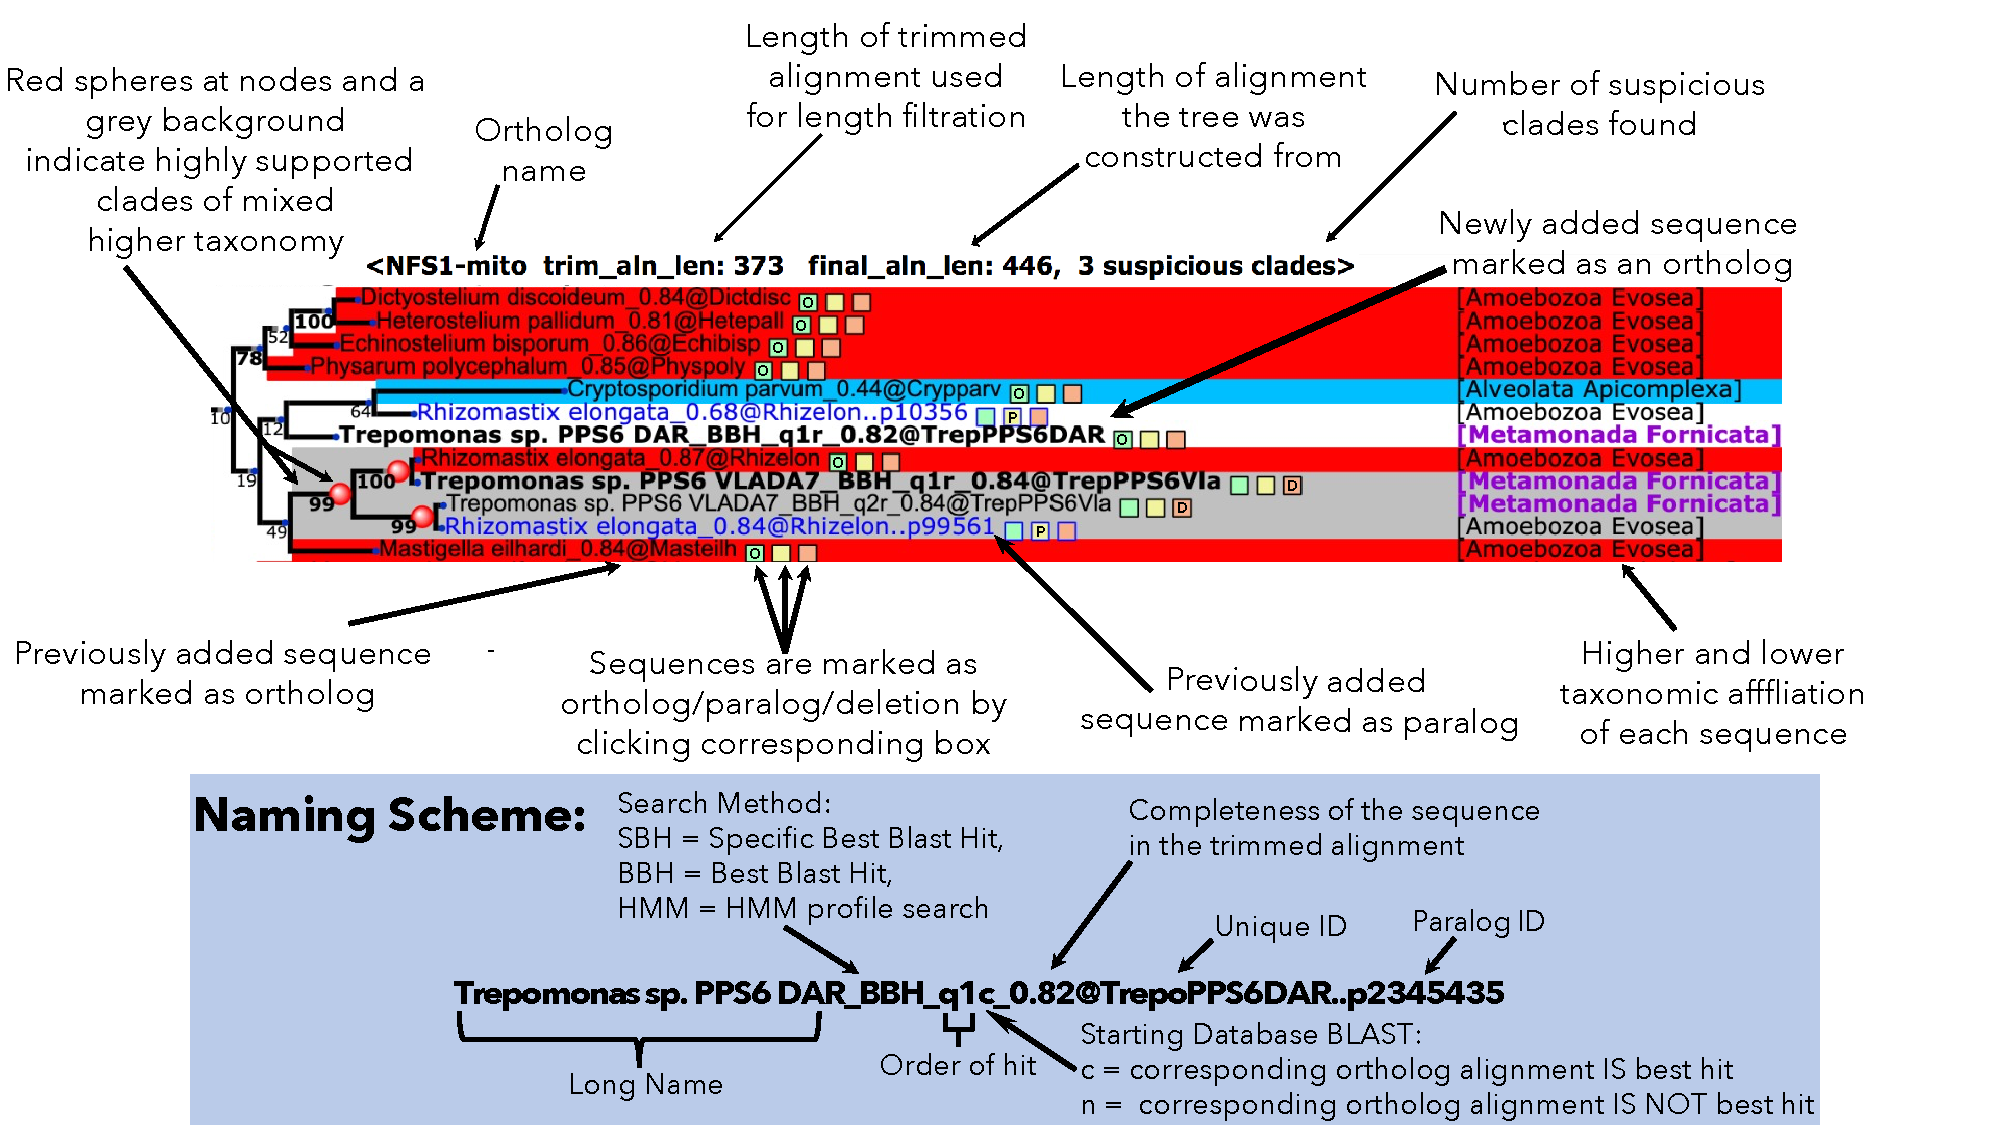
\includegraphics[width=\linewidth]{figures/Martin-Figure-AKT.pdf}
        \caption{Example and explanation of a single gene tree visualized with ParaSorter (above) and of the PhyloFisher sequence header naming scheme (below).}
        \label{Fig:Parasorter}
        \end{figure}
        
        After all decisions have been made click “Save to tsv.” The default name ParaSorter will suggest for the new file will be \{gene\_name\}\_parsed.tsv. The file must have “\{gene\_name\}\_parsed.tsv” naming convention for subsequent steps of the workflow to perform correctly.
    \pagebreak
    \item To backup the database, add new taxa to the database, and implement all decisions made during manual curation with ParaSorter run:
   
   \vspace{0.2cm}
    \code{apply\_to\_db.py [OPTIONS] -i <input\_directory> -fi <fisher\_output\_dir>}
    \vspace{0.2cm}
    
    \begin{description}
        \item Required arguments:
        \begin{description}
            \item -i, -\/-input \hspace{0.2cm} <in\_dir> \hspace{0.2cm} Path to input directory containing parsed tsv labeled \{gene\_name\}\_parsed.tsv
            \item -fi, -\/-fisher\_dir \hspace{0.2cm} <fisher\_output\_dir> \hspace{0.2cm} Path to initial fisher.py output directory
        \end{description}
        \vspace{0.2cm}
        
        \item Optional arguments:
        \begin{description}
            \item -t, -\/-threads \hspace{0.2cm} <N> \hspace{0.2cm} Number of threads
            \item -\/-to\_exclude \hspace{0.2cm} to\_exclude.txt \hspace{0.2cm} Path to .txt file containing Unique IDs of taxa to exclude from dataset addition with one taxon per line
            \begin{itemize}
                \item Example: Unique ID1\\
                \hspace*{1.6cm}Unique ID2
            \end{itemize}
            \item -h, -\/-help \hspace{0.2cm} Show this help message and exit.
        \end{description}
    \end{description}
    \vspace{0.3cm}
    apply\_to\_db.py will first backup the current database/ directory and place the backup in \\
    PhyloFisherDatabase\_v1.0/database/backups. Next, apply\_to\_db.py will append orthologs from input taxa to their corresponding gene files located in /database/orthologs/, append paralogs for input taxa to their corresponding gene files located in /database/paralogs/, and remove sequences marked for deletion. apply\_to\_db.py will update the binary matrix file “db\_ortholog\_occupancy.tsv” for newly added taxa based on decisions made during manual curation. The file “metadata.tsv” will also be updated with information provided for newly added taxa in “input\_metadata.tsv.” Next, apply\_to\_db.py will rebuild the database so sequences from newly added taxa are present in the profile HMMs, the diamond database. This will allow orthologs from the newly added taxa to be used as specific queries in subsequent runs of addition. Finally, apply\_to\_db.py will copy the input proteome of all new taxa that are added to the database to /database/proteomes/.
    
    \item Select a subset of taxa to include in a phylogenomic dataset (OPTIONAL)
    
    \vspace{0.2cm}
    In order to select taxa to be included in the final phylogenomic dataset users can run the script “select\_taxa.py”. This will generate a .tsv file (contents explained below) that will serve to select taxa to include and is used as input for prep\_final\_dataset.py downstream.
    
    \vspace{0.2cm}
    NOTE: If all taxa are to be used in the final phylogenomic analyses this step is not necessary. Skip to step 13 (ALSO OPTIONAL) (to select orthologs to include in the final phylogenomic analyses) or directly to step 14 (if all taxa and all orthologs are to be used in the final phylogenomic analyses).
    
    \vspace{0.2cm}
    To select taxa for the final phylogenomic analyses run:
    
    \vspace{0.2cm}
    \code{select\_taxa.py [OPTIONS]}
    \vspace{0.2cm}
    
    \begin{description}
        \item Optional arguments:
        \begin{description}
            \item -\/-to\_exclude \hspace{0.2cm} taxa\_to\_exclude.txt \hspace{0.2cm} A text file of groups or individual taxa to exclude from the final phylogenomic matrix
            \item -\/-to\_include \hspace{0.2cm} taxa\_to\_include.txt \hspace{0.2cm} a text file that will re-include groups or individual taxa.
            \item -\/-chimeras \hspace{0.2cm} chimeras.tsv \hspace{0.2cm} A .tsv containing a Unique ID, higher and lower taxonomic designations, and the Unique IDs of the taxa to collapse, for each chimera one per line.
            \item -h, -\/-help \hspace{0.2cm} Show this help message and exit
        \end{description}
    \end{description}
    
    \vspace{0.4cm}
    NOTE: Detailed explanation of to the -\/-to\_exclude and -\/-to\_include options and their input files:
    
    \vspace{0.2cm}
    By default all taxa will be included. These options were designed to decrease the amount of manual manipulation of “taxa\_subset.tsv” generated in this first run of “select\_taxa.py.” Manual manipulation will be  necessary if many taxa from the database are to be excluded from the final phylogenomic analysis. Both options take a file created by the user that has one column with an organism’s Unique ID or a taxonomic rank (higher or lower) from the metadata to be excluded or included in downstream steps. The options can be used individually or in conjunction with one another to implement decisions on taxa selection in an automated fashion. For example, if all taxa in the eukaryotic assemblage “Amoebozoa” are to be excluded from downstream phylogenomic analyses provide the -\/-exclude\_taxa option with a file (named anything) that contains “Amoebozoa” as the first entry of the column. This will result in all amoebozoans being marked as “no” in the “Include in Subset” column of “taxa\_subset.tsv” when it is generated. If a user wanted all amoebozoans excluded except \textit{Dictyostelium discoideum} (Unique ID = Dictdisc) provide the -\/-exclude\_taxa option with a file (named anything) that contains “Amoebozoa” as the first entry of the column as before and the -\/-to\_include option with a file (named anything) with “Dictdisc” as the first entry of the column. This will result in all amoebozoans being marked as “no” in the “Include in Subset” column of “taxa\_subset.tsv” except \textit{D}. \textit{discoideum} which will be marked “yes.”
    
    \vspace{0.2cm}
    NOTE: -\/-to\_include is not necessary it only serves to ease the burden of manual taxa selection in cases as outlined above. All taxa are marked to include by default so it is NOT necessary to provide -\/-to\_include with a list of all taxa you wish to include in downstream steps.
    
    \vspace{0.2cm}
    NOTE) Decisions provided to -\/-to\_include will override decisions provided to -\/-to\_exclude so be cautious.
    
    Alternatively, all changes can be made manually by opening “select\_taxa.tsv” and changing taxa designations from “yes” to “no.”
    
    \vspace{0.2cm}
    NOTE) An example input file for the --chimeras option of select\_taxa.py is given below in \autoref{Tab:chimera} below.
    
    \vspace{0.2cm}
                
                \begin{table}[hbt!]
                \centering
                \begin{tabular}{|c|c|c|c|c|c|}
                \hline BrevCHIM & Obazoa & Breviatea & Brevanat & Lenilimo & Pygsbifo \\ \hline
                    \end{tabular}]
                    \caption{Example input .tsv file for the -\/-chimera option of select\_taxa.py. Here a chimera will be made from three breviates in the database. The chimera will have the Unique ID "BrevCHIM", the higher taxonomy "Obazoa", the lower taxonomy "Breviatea" and will be made from Brevanat (\textit{Breviata anathema}), Lenilimo (\textit{Lenisia limosa}), Pygsbifo (\textit{Pygsuia biforma}).}
                    \label{Tab:chimera}
                \end{table}
    
    \vspace{0.2cm}
    \begin{description}
        \item Default select\_taxa.py output:
        \begin{itemize}
            \item a .tsv file “select\_taxa.tsv”  with five columns:
            \begin{enumerate}[label=\arabic*.]
                \item Unique ID
                \item Higher Taxonomy
                \item Lower Taxonomy
                \item Completeness (percentage of orthologs) from the database present in the taxon
                \item Include in Subset
            \end{enumerate}
        \item a plot showing completeness (number of orthologs) in each taxon. Groups of taxa are colored by level of completeness in increments of 10\% (\autoref{Fig:taxacomp}).
        \end{itemize}
    \end{description}
  
        \begin{figure}[H]
        \centering
        \includegraphics[width=\linewidth]{figures/taxa_comp.pdf}
        \caption{Plot produced by select\_taxa.py. Taxa Unique IDs are shown at the bottom of the figure across the x-axis. The percentage of total orthologs present in a taxon (completeness) is shown on the y-axis. The total number of taxa is shown across the top of the figure on the x-axis. The bars are colored by level of completeness in increments of 10\%. Legend explaining color coding is shown in the top right of the figure.}
        \label{Fig:taxacomp}
        \end{figure}
    
    \item Select orthologs to be included in the final phylogenomic dataset (OPTIONAL).
    
    \vspace{0.2cm}
    NOTE: If all orthologs are to be included in the final phylogenomic dataset this step is not necessary. Skip to step 14.
    
    \vspace{0.2cm}
    To select orthologs to be included in the final phylogenomic dataset run:
    
    \vspace{0.2cm}
    \code{select\_orthologs.py [OPTIONS]}
    \vspace{0.2cm}
    
    \begin{description}
        \item Optional arguments:
        \begin{description}
            \item -\/-out\_group \hspace{0.2cm} out\_group.txt \hspace{0.2cm} Path to text file containing out group taxa Unique IDs.
            \item -n, -\/-gene\_number \hspace{0.2cm} <N> \hspace{0.2cm} Number of genes for analysis
            \item -c, -\/-percent\_complete \hspace{0.2cm} <N> \hspace{0.2cm} Threshold for percent completeness
            \item -h, -\/-help \hspace{0.2cm} Show this help message and exit
        \end{description}
        
        \vspace{0.2cm}
        \item select\_orthologs.py  output:
        \begin{itemize}
            \item a tsv file “select\_orthologs.tsv” with three either three or five columns:
            \begin{enumerate}[label=\arabic*.]
                \item Ortholog - ortholog name
                \item Total Completeness - percentage of all taxa to be included in the final phylogenomic dataset the ortholog is present in.
                \item In-Group Completeness (only present if -\/-out\_group option is utilized) -percentage of In-group taxa only to be included in the final phylogenomic dataset the ortholog is present in.
                \item Out-Group Completeness (only present if -\/-out\_group option is utilized) - percentage of Out-Group taxa only to be included in the final phylogenomic dataset the ortholog is present in.
                \item Include in Subset
            \end{enumerate}
        \item a plot showing completeness (number of taxa) of each gene. Groups of genes are colored by level of completeness in increments of 10\% (\autoref{Fig:orthocomp}). 
        \end{itemize}
    \end{description}
        
        \begin{figure}[H]
        \centering
        \includegraphics[width=\linewidth]{figures/ortho_comp_big.pdf}
        \caption{Plot produced by select\_orthologs.py. Ortholog names are shown at the bottom of the figure across the x-axis. The percentage of total taxa present in an ortholog (completeness) is shown on the y-axis. The total number of genes is shown across the top of the figure on the x-axis. The bars are colored by level of completeness in increments of 10\%. Legend explaining color coding is shown in the top right of the figure.}
        \label{Fig:orthocomp}
        \end{figure}
        

    \item Collect orthologs and taxa to be included in the final phylogenomic dataset
    
    \vspace{0.2cm}
    To do this run:
    
    \vspace{0.2cm}
    \code{prep\_final\_dataset.py [OPTIONS]}
    \vspace{0.2cm}
    
    \begin{description}
        \item Optional arguments:
        \begin{description}
            \item -o, -\/-output \hspace{0.2cm} <out\_dir>  \hspace{0.2cm} Path to user-defined output directory
            \begin{itemize}
                \item default ./prep\_final\_dataset\_<M.D.Y>
            \end{itemize}
            \item -h, -\/-help \hspace{0.2cm} Show this help message and exit
        \end{description}
        
    \vspace{0.2cm}
    \item{Default prep\_final\_dataset.py  output:}
    \begin{itemize}
        \item a directory called prep\_final\_dataset\_<M.D.Y> that contains:
        \begin{itemize}
            \item a fasta file of each ortholog selected to be in the final phylogenomic dataset each containing only taxa selected to be in the final phylogenomic dataset.
        \end{itemize}
    \end{itemize}
    \end{description}
    
    \item Trim, align, and concatenate orthologs into a super-matrix.
    
    \vspace{0.2cm}
    To do this run:
    
    \vspace{0.2cm}
    \code{matrix\_constructor.py [OPTIONS] -i <input\_directory>}
    \vspace{0.2cm}
    
    \begin{description}
        \item Required arguments:
        \begin{description}
            \item -i, -\/-input \hspace{0.2cm} <in\_dir> \hspace{0.2cm} Path to prep\_final\_dataset\_<M.D.Y>
        \end{description}
        \vspace{0.2cm}
        

        \item Optional arguments:
        \begin{description}
            \item -f, -\/-out\_format \hspace{0.2cm} <format> \hspace{0.2cm} Desired format of the output matrix
            \begin{itemize}
                \item Options: fasta, phylip,  phylip-relaxed, or nexus.
                \item Default: fasta
            \end{itemize}
            \item -if, -\/-in\_format \hspace{0.2cm} <format> \hspace{0.2cm} format of the input files.
            \begin{itemize}
                \item Options: fasta, phylip, phylip-relaxed, or nexus.
                \item Default: fasta
            \end{itemize}
            \item -c, -\/-concatenation\_only \hspace{0.2cm} Only concatenate alignments. Filtering, alignment, and trimming are not performed automatically.
            \item -t, -\/-threads \hspace{0.2cm} <N> \hspace{0.2cm} Desired number of threads to be utilized.
            \begin{itemize}
                \item Default: 1
            \end{itemize}
            \item -o, -\/-output \hspace{0.2cm} <out\_dir> \hspace{0.2cm} Path to user-defined output directory
            \begin{itemize}
                \item Default: ./matrix\_constructor\_out\_<M.D.Y>
            \end{itemize}
            \item -p, -\/-prefix \hspace{0.2cm} <prefix> \hspace{0.2cm} Prefix of input files
            \begin{itemize}
                \item Default: NONE
                \item Example: path/to/input/prefix*
            \end{itemize}
            \item -s, -\/-suffix \hspace{0.2cm} <suffix> \hspace{0.2cm} Suffix of input files
            \begin{itemize}
                \item Default: NONE
                \item Example: path/to/input/*suffix
            \end{itemize}
            \item -h, -\/-help \hspace{0.2cm} Show this help message and exit
        \end{description}
    \end{description}
    \vspace{0.2cm}
    \begin{description}
    \item Default matrix\_constructor.py output:
    \begin{itemize}
        \item a directory called “matrix\_constructor\_out\_<M.D.Y>” containing:
        \begin{itemize}
            \item a directory “prequal” that contains:
            \begin{itemize}
                \item \{gene\_name\}.aa - unaligned gene file used as PREQUAL input
                \item \{gene\_name\}.aa.filtered - output of PREQUAL. Used as input for MAFFT in subsequent length filtration step.
                \item \{gene\_name\}.aa.filtered.PP - output of PREQUAL.\textsuperscript{\#\#}
                \item \{gene\_name\}.aa.warning - output of PREQUAL.\textsuperscript{\#\#}
            \end{itemize}
        \item a directory “mafft” that contains:
        \begin{itemize}
            \item \{gene\_name\}.aln - output of  of MAFFT and input for Divvier.
            \item \{gene\_name\}.aln.PP - output of PREQUAL.\textsuperscript{\#\#}
        \end{itemize}
        \item a directory “divvier” that contains:
        \begin{itemize}
            \item \{gene\_name\}.aln.partial.fas - output of Divvier and input for timAl.
        \end{itemize}
        \item a directory “trimAl” that contains:
        \begin{itemize}
            \item \{gene\_name\}.gt80trimAl.fas - output of trimAl. Trimmed alignments, in FASTA format, that will be used for concatenation.
        \end{itemize}
        \item indices.tsv - a tab separated file with three columns outlining the single gene boundaries in the supermatrix:
        \begin{enumerate}[label=\arabic*.]
            \item Gene - name of the gene
            \item Start - first position of the gene within the super matrix
            \item Stop - last position of the gene within the super matrix
        \end{enumerate}
        \item matrix.<fas | nex | phy> - the concatenated super matrix of all genes in the provided input directory in the specified file format.
        \item matrix\_constructor\_stats.tsv - a tab separated file with two columns:
        \begin{enumerate}[label=\arabic*.]
            \item Taxon -Unique ID of taxon in the database
            \item Percent Missing Data - percentage of unoccupied sites within the concatenated matrix.
        \end{enumerate}
        \end{itemize}
    \end{itemize}
        \vspace{0.2cm}
        \textsuperscript{\#\#} - These are standard PREQUAL output files for each gene that PhyloFisher has appended the corresponding gene name to. See the \href{http://amoeba.msstate.edu/phylofisher/pdfs/prequal.pdf}{PREQUAL documentation} for a thorough explanation of their contents.
        \vspace{0.2cm}
    \end{description}
    \end{enumerate}
    
    \pagebreak
    
    \section{UTILITIES}
    \subsection{Overview}
    While the above processes will allow users to develop a phylogenomic dataset and infer single gene and phylogenomic trees using whatever best practices are available to them, many more analyses are often used to examine the effects of aspects of the data. Phylogenomic analyses are often accompanied by additional analyses in which users manipulate their phylogenomic dataset or examine the dataset in a different fashion to reveal artifacts in their data. Here we provide users with simple programs to perform some of the most often employed tactics. 
    
    \begin{description}
    \item \textbf{aa\_comp\_calculator.py:} Calculates amino acid composition and uses euclidean distances to hierarchically cluster these data, in order to examine if amino acid composition may bias the groupings that were inferred in a phylogenomic tree. See \cite{brown_phylogenomics_2018} for an example.
    
    \item \textbf{astral\_runner.py:} Generates input files and infers a coalescent-based species tree given a set of single ortholog trees and bootstrap trees using ASTRAL-III (\cite{zhang_astral-iii_2018}). 

    \item \textbf{backup\_restoration.py:} Restores a previous version of the database from  the directory backups/.

    \item \textbf{bipartition\_examiner.py:} Calculates the observed occurrences of clades of interest in bootstrap trees.

    \item \textbf{build\_database.py:} used to format custom databases for use in the PhyloFisher workflow. This utility is also used to rename taxa in either the provided database or a custom database.

    \item \textbf{explore\_database.py:} Used to examine the composition of the database using taxonomic terms as search queries.

    \item \textbf{fast\_site\_remover.py:} The fastest evolving sites are expected to be the most prone to phylogenetic signal saturation and systematic model misspecification in phylogenomic analyses. This tool will remove the fastest evolving sites within the phylogenomic supermatrix in a stepwise fashion, leading to a user defined set of new matrices with these sites removed.

    \item \textbf{fast\_taxa\_remover.py:} Removes the fastest evolving taxa, based on branch length. This tool will remove the fastest evolving taxa within the phylogenomic supermatrix in a stepwise fashion, leading to a user defined set of new matrices with these taxa removed.

    \item \textbf{genetic\_code\_examiner.py:} Checks stop-to-sense and sense-to-sense codon reassignment signal in transcriptome/genome data. This script is using the advantage of the phylogenetically broad database accompanying our software. The first step is the creation of multiple sequence alignments from all fasta files containing manually curated orthologous sequences. This step can take some time but it is necessary only for the first run of genetic\_code.py. In the next step, tblastn searches with orthologs from selected related organism/s in the database are performed against the given transcriptome/genome (with 1e-30 default e-value). For all genes, the best scoring hit is investigated for “good quality positions''. Such positions are located at least 6 amino acids from the beginning or end of the blast alignment and the number of low scoring mismatches (normally denoted by spaces in blast middle line) in close proximity to these positions (+- 3 amino acids) is less than 3. Corresponding positions from the query are then analyzed in previously prepared multiple sequence alignments and information about well-conserved amino acids (in more than 70\% of organisms, default) is collected and connected to the underlying codon from transcriptome/genome. Codons which show evidence for signals different from the standard genetic code signal are then visualized in the form of bar plots (occurrence of conserved amino acids). Thanks to the evolutionary well-conserved nature of proteins in our database, realigning all sequences again with provided input nucleotide data is not necessary. This script performs well with genomic and transcriptomic data. Analysis of one transcriptome/genome should usually take less than 5 minutes on an average personal computer. It has to be mentioned that alternative genetic code signal from multiple sequence alignments is only one way to analyze this phenomenon and tRNAs should be investigated as well if possible.

    \item \textbf{heterotachy.py:} Within-site rate variation (heterotachy) (\cite{Lopez-Heterotachy}) has been shown to cause artificial relationships in molecular phylogenetic reconstruction (\cite{Inagaki-Heterotachy}).  This tool will remove the most heterotachious sites within a phylogenomic supermatrix in a stepwise fashion, leading to a user defined set of new matrices with these sites removed.

    \item \textbf{mammal\_modeler.py:} Generates a MAMMaL site heterogeneous model from a user input tree and supermatrix with estimated frequencies for a user defined number of classes. This program creates a set of temporary files from the user provided input that MAMMaL is able to handle. The output is a heterogeneous model in Nexus format that is usable in IQtree using options (-m LG+ESmodel+G -mdef esmodel.nex). This program outputs by default a 61 class mixture model with 60 site frequency classes and the overall amino acid frequencies (+F) of the phylogenomic dataset. Also please note that when using this program we hard-code the “not using likelihood weighting” option. This is because using likelihood weighting will cause issues in the calculation of likelihood weights in sparse phylogenomic matrices. The problem is that there may be pairs of sequences that have no sites in common. Specifically, the proportion of times an amino acid occurs for the pair of sequences becomes NA because the denominator is 0 (calculation is [p\_\{aa;sj\}] in Eqn (5) of the \cite{susko_accelerated_2018}) (Ed Susko personal communication). 

    \item \textbf{purge.py:} This tool is used for deleting taxa and/or taxonomic groups from the database and metadata permanently. 

    \item \textbf{random\_resampler.py:} This tool randomly resamples the gene set into a set of new matrices that are subsamples of the super matrix. It constructs supermatrices from randomly sampled genes with user defined options such as the confidence interval sampling all genes in a random fashion and the percentage of subsampling a user requires per sampling step. This method was used in \cite{brown_phylogenomics_2018} as an example. 

    \item \textbf{rtc\_binner.py:} Calculates the relative tree certainty score (RTC) in RAxML \cite{stamatakis_raxml_2014} of each single ortholog tree and bins them based on their RTC scoring into top 25\%, 50\%, and top 75\% sets. Supermatrices are constructed from these bins of orthologs. 

    \item \textbf{SR4\_class\_recoder.py:} To minimize phylogenetic saturation this tool recodes input supermatrix into the four-character state scheme of SR4 (\cite{Susko-SR4}), based on  amino acid classification.

    \item \textbf{taxon\_collapser.py:} Allows users to combine multiple operational taxonomic units into one single taxon. For example if a user has multiple single cell libraries from a taxon or multiple strains of the same species (or genus etc.), a user may decide to  collapse all these strains/libraries into a single taxon. 
    \end{description}
    
    \subsection{Example Usages of Utilities:}

        
        \subsubsection{Calculate the amino acid composition of an input matrix.}
        
        \begin{description}
    
            \vspace{0.2cm}
            \item \code{aa\_comp\_calculator.py [OPTIONS] -i <input\_matrix>}
            \vspace{0.2cm}
    
            \begin{description}
                \item Required arguments:
                \begin{description}
                    \item -i, -\/-input matrix \hspace{0.2cm} Path to input matrix for analysis
                \end{description}
            \end{description}
            \vspace{0.2cm}
            \begin{description}
                \item Optional arguments:
                \begin{description}
                    \item -o, -\/-output \hspace{0.2cm} <out\_dir> \hspace{0.2cm} Path to user-defined output directory
                    \begin{itemize}
                        \item Default: ./aa\_comp\_calculator\_out\_<M.D.Y>
                    \end{itemize}
                    \item -h, -\/-help \hspace{0.2cm} Show this help message and exit
                \end{description}
            \end{description}
        
        \vspace{0.2cm}
            \begin{description}
                \item Default aa\_comp\_calculator.py output:
                \begin{itemize}
                    \item a directory “aa\_comp\_calculator\_output\_<M.D.Y>” that contains:
                    \begin{itemize}
                        \item a tab separated file “aa\_comp.tsv” with 21 columns:
                        \begin{enumerate}[label=\arabic*.]
                            \item “Taxon” - short name of taxon in dataset
                            \item Each of the following 20 columns are labeled with the IUPAC single letter abbreviation for each standard amino acid. The values in rows are the proportion of the corresponding amino acid in the sequence data for a taxon in the input file.
                        \end{enumerate}
                        \item AA\_Composition\_Hierarchical\_Clustering.pdf” - a dendrogram built using pairwise distances calculated by Ward’s criterion between taxa after hierarchical clustering based on amino acid composition in pdf format \autoref{Fig:aahclust}.
                    \end{itemize}
                \end{itemize}
            \end{description}
        \end{description} 
        
        \begin{figure}[H]
        \centering
        \includegraphics[width=\linewidth]{figures/aa_comp_calculator.pdf}
        \caption{Plot produced by aa\_comp\_calculator. The plot is built using pairwise distances calculated by Ward’s criterion between taxa after hierarchical clustering based on amino acid composition as performed in \cite{brown_phylogenomics_2018}. Leaves are labeled and colored according to higher taxonomy of taxa in the provided alignment.}
        \label{Fig:aahclust}
        \end{figure}
        
        \vspace{0.5cm}
        
        \subsubsection{Generate input files and infer a coalescent-based species tree with ASTRAL-III.}
        \begin{description}
        
        
            \vspace{0.2cm}
            \item \code{astral\_runner.py [OPTIONS] -i <input\_directories>}
            \vspace{0.2cm}
        
            \begin{description}
                \item Required arguments:
                \begin{description}
                    \item -i, -\/-input \hspace{0.2cm} <input\_directory> \hspace{0.2cm} Path to directory containing single gene trees and their corresponding bootstrap value files.
                \end{description}
                \vspace{0.2cm}
                \item Optional arguments:
                \begin{description}
                    \item -o, -\/-output \hspace{0.2cm} <out\_dir> \hspace{0.2cm} Path to user-defined output directory
                    \begin{itemize}
                        \item Default: ./astral\_runner\_<M.D.Y> 
                    \end{itemize}
                    \item -p, -\/-prefix \hspace{0.2cm} <prefix> \hspace{0.2cm} Prefix of input files
                    \begin{itemize}
                        \item Default: NONE
                        \item Example: path/to/input/prefix*
                    \end{itemize}
                    \item -s, -\/-suffix \hspace{0.2cm} <suffix> \hspace{0.2cm} Suffix of input files
                    \begin{itemize}
                        \item Default: NONE
                        \item Example: path/to/input/*suffix
                    \end{itemize}
                    \item -h, -\/-help \hspace{0.2cm} Show this help message and exit.
                \end{description}
            \end{description}
            \vspace{0.2cm}
            \begin{description}
                \item Default astral\_runner.py output:
                \begin{itemize}
                    \item a file all\_sgt.tre that contains:
                    \begin{itemize}
                        \item all single gene trees provided in Newick format
                    \end{itemize}
                    \item a file bs\_files.txt that contains:
                    \begin{itemize}
                        \item paths to all ML bootstrap files
                    \end{itemize}
                    \item a file astral\_BS.out that contains:
                    \begin{itemize}
                        \item 100 bootstrapped replicate trees
                        \item A greedy consensus of the 100 bootstrapped replicate trees
                        \item The “main” ASTRAL tree
                    \end{itemize}
                \end{itemize}
            \end{description}
        \end{description}
        \vspace{0.2cm}
        NOTE: Users may choose to use the trees generated by sgt\_constructor.py using the ortholog files generated by the matrix\_constructor.py. For example, "sgt\_constructor.py --trees\_only -i matrix\_constructor\_out\_<M.D.Y>/trimal/ -o <above, directory of your choice>/". If users construct trees via this method, example run is "rtc\_binner.py -i <directory of your choice>/RAxML/ -st gt80trimal.tre -s gt80trimal".
        
        
        \vspace{0.5cm}
        
        \subsubsection{Restore the database from a backup.}
        \begin{description}
    
    
            \vspace{0.2cm}
            \item \code{backup\_restoration.py [OPTIONS] -d <path/to/database/>}
            \vspace{0.2cm}
        
            \begin{description}
                \item Required arguments:
                \begin{description}
                    \item -d, -\/-database \hspace{0.2cm} <db\_dir> \hspace{0.2cm} Path to database directory.
                \end{description}
                \vspace{0.2cm}
                \item Optional arguments:
                \begin{description}
                    \item -\/-list\_backups \hspace{0.2cm} List available backups to restore from.
                    \item -\/-restore \hspace{0.2cm} <N> \hspace{0.2cm} Number of backup to restore from.
                    \item -h, -\/-help \hspace{0.2cm} Show this help message and exit.
                \end{description}
            \end{description}
        \end{description}
        
        \vspace{0.5cm}
        
        \subsubsection{Calculate and plot the observed occurrences of clades of interest in bootstrap trees.}
        \begin{description}
            

            \vspace{0.2cm}
            \item \code{bipartition\_examiner.py [OPTIONS] -b <input\_MLBS\_files> -g groups.txt}
            \vspace{0.2cm}
            
            \begin{description}
                \item Required arguments:
                \begin{description}
                    \item -b, -\/-bs\_files \hspace{0.2cm} <infile> \hspace{0.2cm} A file that contains paths to sets of bootstrap tree files. One file name per line (\autoref{Tab:bsfiles}). Results from files will be plotted in the order they were provided
                    \item -g, -\/-groups \hspace{0.2cm} <infile> \hspace{0.2cm} A file containing taxonomic groups/relationships of interest one per line (\autoref{Tab:groups})
                \end{description}
            \end{description}
            \vspace{0.2cm}
            \begin{description}
                \item Optional arguments:
                \begin{description}
                    \item -o, -\/-output \hspace{0.2cm} <out\_dir> \hspace{0.2cm} Path to user-defined output directory
                    \begin{itemize}
                        \item Default: ./bipartition\_examiner\_out\_<M.D.Y>
                    \end{itemize}
                    \item -\/-bar\_plot \hspace{0.2cm} Plot categorical data as a barplot
                    \begin{itemize}
                        \item Default: Plot series data as a line graph.
                    \end{itemize}
                    \item -h, -\/-help \hspace{0.2cm} Show this help message and exit.
                \end{description}
            \end{description}
            \vspace{0.2cm}
            \begin{description}
                \item bipartion\_examiner.py output:
                \begin{itemize}
                    \item bipartion\_examiner.pdf  - a plot (line graph or histogram) with MLBS values on the y-axis file names on the x-axis. Groups of interest are color coded.
                    \item bipartion\_examiner.tsv - a .tsv file that contains the values plotted in bipartion\_examiner.pdf
                \end{itemize}
            \end{description}
        \end{description}
  
        \vspace{0.2cm}

        \begin{center}
        \begin{table}[H]
        \centering
        \begin{tabular}{ |c| } 
        \hline
        /home/myworkingdirectory/MLbootstrap.experiment1 \\
        \hline
        /home/myworkingdirectory/MLbootstrap.experiment2 \\
        \hline
        /home/myworkingdirectory/MLbootstrap.experiment3 \\
        \hline
        \end{tabular}
        \captionsetup{width=.89\textwidth}
        \caption{Example input file provided to bipartition\_examiner.py via the -b/-\/-bs\_files options providing the location of input sets of bootstrap trees. The results will be plotted in the order the files were provided.}
        \label{Tab:bsfiles}
        \end{table}
        \end{center}
    
        \begin{center}
        \begin{table}[H]
        \centering
        \begin{tabular}{ |l| } 
        \hline
        Amoebozoa \\
        \hline
        Amoebozoa+Obazoa+CRuMs \\
        \hline
        Fungi+Metazoa \\
        \hline
        Homosapi+Gallgall \\
        \hline
        Fungi:Sacccere,Candalbi,Aspefumi,Coprcine \\
        \hline
        \end{tabular}
        \captionsetup{width=.89\textwidth}
        \caption{Example input file provided to bipartition\_examiner.py via the -g/-\/-groups options that lists the groups of interest to be examined in the sets of bootstrap trees. If the data has been processed through the PhyloFisher workflow and a metadata.tsv exists detailing the higher and lower taxonomy of each taxon in the dataset then these taxonomic terms can be utilized here along with individual Unique IDs to examine support for relationships of interest. \textbf{In summary, lines 1-4 are only if the data has been processed through the PF workflow and a metadata file exists. If bipartion\_examiner.py is being used as a stand-alone tool each group of interest will have to be defined as in line 5.} Here the group label (Fungi) is followed by a colon and sequence headers (ex. Sacccere) of all taxa in the group are listed and separated by commas.}
        \label{Tab:groups}
        \end{table}
        \end{center}
        
        \vspace{0.5cm}
        
        \subsubsection{Construct a custom database or update taxonomy in a database.}
        \label{sec:builddb}
        \begin{description}
        
        
            \vspace{0.2cm}
            \item \code{build\_database.py [OPTIONS]}
            \vspace{0.2cm}
            
            \begin{description}
                \item Optional arguments"
                \begin{description}
                    \item -t, -\/-threads \hspace{0.2cm} <N> \hspace{0.2cm} Number of threads
                    \begin{itemize}
                        \item Default:1
                    \end{itemize}
                    \item -n, -\/-no\_og\_file \hspace{0.2cm} Do not make Gene OG file
                    \item -o, -\/-og\_threshold \hspace{0.2cm} 0.X (0-1) proportion of sequences that must hit an OrthoMCL orthogroup for the group to be assigned.
                    \begin{itemize}
                        \item Default: 0.1 (10\%)
                    \end{itemize}
                    \item -\/-rename \hspace{0.2cm} <to\_rename.tsv> \hspace{0.2cm} Rename taxa in the database. Input is a tab-delimted file (.tsv) containing the Old Unique ID, New Unique ID, and New Long Name (\autoref{Tab:rename}).
                    \item -h, -\/-help \hspace{0.2cm} Show this help message and exit
                \end{description}
            \end{description}
            \vspace{0.2cm}
            NOTE: build\_database.py must be run within PhyloFisherDatabase\_v1.0/database\
            \vspace{0.2cm}
            \begin{description}
                \item build\_database.py output:
                \begin{itemize}
                    \item a directory “profiles” that contains:
                    \begin{itemize}
                        \item profile HMMs of all ortholog files from the custom database
                    \end{itemize}
                    \item a directory “datasetdb” that contains:
                    \begin{itemize}
                        \item a diamond blast database of the orthologs from the custom database
                    \end{itemize}
                    \item a directory “paralogs” - This empty directory is created if no paralogs directory exists initially
                    \item a tab separated file “gene\_og” with two columns:
                    \begin{enumerate}
                        \item Name of gene from the custom database
                        \item OrthoMCL orthogroup identification number(s) assigned to a gene from the custom database separated by commas.
                    \end{enumerate}
                \end{itemize}
            \end{description}
            \vspace{0.2cm}
            \item What occurred:
            \begin{itemize}
                \item The script build\_database.py will:
                \begin{itemize}
                    \item align the provided set of orthologs using MAFFT and create profile HMMs for each gene alignment using the “hmmbuild” utility from the HMMER3 package. These profiles will be used in the ortholog “fishing” algorithms implemented in fisher.py.
                    \item build a diamond blast database from the set of provided orthologs for use in the ortholog “fishing” algorithms implemented in fisher.py.
                    \item assign OrthoMCL orthogroup number(s) to each ortholog for use in the ortholog “fishing” algorithms implemented in fisher.py.
                    \begin{itemize}
                        \item OrthoMCL orthogroup numbers are assigned by using all sequences in a provided gene file as queries in a BLAST search against the OrthoMCL v. 5.0 database. If a user defined percentage (default = 10\%) of sequences hit an OrthoMCL orthogroup with a significance threshold of evalue < 1e -10 then that Orthogroup is assigned to the gene.
                        \item More than one OrthoMCL orthogroup numbers can be assigned to one gene.
                        \item If the provided gene alignment is assigned “no group” in OrthoMCL the gene cannot be used in the PhyloFisher workflow.
                        \item If the gene is assigned a bacterial OrthoMCL orthogroup the gene cannot be used in the PhyloFisher workflow.
                    \end{itemize}
                \end{itemize}
            \end{itemize}
        \vspace{0.2cm}
        NOTE: OrthoMCL orthogroup assignment hinges on integrity of ortholog choices in the starting ortholog files provided. If paralogs are unknowingly present in the provided ortholog alignments the paralogs will likely be prioritized by the fisher algorithm. To investigate the level of paralogy of genes in a custom database, we strongly recommend users re-add all taxa in their custom database using the main workflow of PhyloFisher. After an initial run through the main PhyloFisher workflow that includes manual curation, we recommend users rerun build\_dataset.py to update profile HMMs, and blast databases to promote highest level of accuracy by the fisher algorithm in subsequent runs.
        \end{description}
        \vspace{0.5cm}
        \begin{table}[H]
        \centering
        \csvreader[
            tabular=|{c}|{c}|{c}|,
            table head=  \hline Old Unique ID & New Unique ID & New Full Name \\ \hline,
            late after last line=\\\hline,
            ]{tables/rename.csv}{}%
            {\csvcoli & \csvcolii & \csvcoliii}
            \caption{Example input file for the -\/-rename flag of build\_database.py. Here \textit{Pleurochrysis carterae} (Unique ID = Pleucart) is being renamed to Chrysotila carterae (Unique ID = Chrycart) in the database.}
            \label{Tab:rename}
        \end{table}
        
        \vspace{0.5cm}
        
        \subsubsection{Examine the composition of the database using taxonomic terms as search queries.}
        \begin{description}
        
            \vspace{0.2cm}
            \item \code{explore\_database.py [OPTIONS]}
            \vspace{0.2cm}
            
            \begin{description}
                \item Optional arguments:
                \begin{description}
                    \item -d, -\/-database \hspace{0.2cm} <db\_dir> \hspace{0.2cm} Path to the database directory if config.py has not been run.
                    \item -t, -\/-higher\_taxonomy \hspace{0.2cm} Show higher taxonomy and number of taxa in each group in the database.
                    \item -l, -\/-lower\_taxonomy \hspace{0.2cm} Show lower taxonomy and number of taxa in each group in the database.
                    \item -r, -\/-get\_higher \hspace{0.2cm} <HigherTax> \hspace{0.2cm} Return table with all taxa assigned the given higher taxonomy that displays the UniqueID, Long Name, Higher and Lower taxonomy, the number of orthologs, and the number of paralogs present in the database.
                    \item -w, -\/-get\_lower \hspace{0.2cm} <LowerTax> \hspace{0.2cm} Return table with all taxa assigned the given lower taxonomy that displays the UniqueID, Long Name, Higher and Lower Taxonomy, the number of orthologs, and the number of paralogs present in the database.
                    \item -o, -\/-get\_org \hspace{0.2cm} <UniqueID> \hspace{0.2cm} For the given Unique ID returns the Long Name, Higher and Lower Taxonomic Designation, Data Type, Orthologs (number present in the database for the taxon), Paralogs (number present in the database for the taxon), and the Accession.
                \end{description}
            \end{description}
        \end{description}
        
        \vspace{0.5cm}
        
        \subsubsection{Remove the fastest evolving sites within a phylogenomic supermatrix in a stepwise fashion.}
        \begin{description}
        
            \vspace{0.2cm}
            \item \code{fast\_site\_remover.py [OPTIONS] -m <input\_matrix> -tr <input\_tree>}
            \vspace{0.2cm}
            
            \begin{description}
                \item  Required arguments:
                \begin{description}
                    \item  -m, -\/-matrix \hspace{0.2cm} <matrix.fas|nex|phy> \hspace{0.2cm} Path to matrix
                    \item -tr, -\/-tree	\hspace{0.2cm} <input.tre> Path to tree in Newick format
                \end{description}
            \end{description}
            \vspace{0.2cm}
            \begin{description}
                \item Optional arguments:
                \begin{description}
                    \item -s, -\/-step\_size \hspace{0.2cm} <N> \hspace{0.2cm} Size of removal step (i.e., 3000 sites removed) to exhaustion
                    \begin{itemize}
                        \item Default: 3000
                    \end{itemize}
                    \item -f, -\/-out\_format \hspace{0.2cm} <format> \hspace{0.2cm} Desired format of the output matrices
                    \begin{itemize}
                        \item Options: fasta, nexus, phylip (names truncated at 10 characters), or phylip-relaxed (names are not truncated)
                        \item Default: fasta
                    \end{itemize}
                    \item -o, -\/-output \hspace{0.2cm} <out\_dir> \hspace{0.2cm} Path to user-defined output directory
                    \begin{itemize}
                        \item Default: ./fast\_site\_removal\_out\_<M.D.Y> with sub-directories:
                        \begin{itemize}
                            \item steps\_N
                        \end{itemize}
                    \end{itemize}
                    \item -h, -\/-help \hspace{0.2cm} Show this help message and exit
                \end{description}
            \end{description}
            \vspace{0.2cm}
            \begin{description}
                \item fast\_site\_remover.py output:
                \begin{itemize}
                    \item a directory called ./fast\_site\_removal\_out\_<M.D.Y> with:
                    \begin{itemize}
                        \item sub-directories steps\_<N> (N=step size) that contain:
                        \begin{itemize}
                            \item alignment files of the input matrix with N fastest sites removed iteratively until exhaustion
                        \end{itemize}
                        \item a file DE.dat\textsuperscript{\&\&}
                        \item a file rate\textsuperscript{\&\&}
                        \item dist\_est.ctl\textsuperscript{\&\&}
                    \end{itemize}
                \end{itemize}
            \end{description}
           \textsuperscript{\&\&} These are standard dist\_est input/output files. See the \href{http://amoeba.msstate.edu/phylofisher/pdfs/distest.pdf}{dist\_est documentation} for a more detailed explanation of their contents.
        \end{description}
        
        \vspace{0.5cm}
        
        \subsubsection{Remove the fastest evolving taxa from a matrix based on branch length.}
        \begin{description}
        
            \vspace{0.2cm}
            \item \code{fast\_taxa\_remover.py [OPTIONS] -m <input\_matrix> -tr <input\_tree>}
            \vspace{0.2cm}
            
            \begin{description}
                \item Required arguments:
                \begin{description}
                    \item -m, -\/-matrix \hspace{0.2cm} <matrix.fas|nex|phy> \hspace{0.2cm} Path to input matrix
                    \item -tr, -\/-tree \hspace{0.2cm} <tree> \hspace{0.2cm} Path to input tree
                    \item -i, -\/-iterations \hspace{0.2cm} <N> \hspace{0.2cm} Number of iterations
                    \item -or, -\/-ortholog\_files  \hspace{0.2cm} Path to directory containing the individual ortholog files. This will be the path to prep\_final\_dataset\_<M.D.Y> if used within the main PhyloFisher workflow.
                \end{description}
            \end{description}
            \vspace{0.2cm}
            \begin{description}
                \item Optional arguments:
                \begin{description}
                    \item -in\_format \hspace{0.2cm} <format> \hspace{0.2cm} Input matrix format
                    \begin{itemize}
                        \item Options: fasta, phylip (names truncated at 10 characters), phylip-relaxed (names are not truncated), or nexus
                        \item Default: fasta
                    \end{itemize}
                    \item -out\_format \hspace{0.2cm} <format> \hspace{0.2cm} Desired output format.
                    \begin{itemize}
                        \item Options: fasta, phylip (names truncated at 10 characters), phylip-relaxed (names are not truncated), or nexus
                        \item Default: fasta
                    \end{itemize}
                    \item -s, -\/-step\_size \hspace{0.2cm} <N> \hspace{0.2cm} Number taxa removed per iteration
                    \begin{itemize}
                        \item Default: 1
                    \end{itemize}
                    \item -o, -\/-output \hspace{0.2cm} <out\_dir> \hspace{0.2cm} Path to user-defined output directory
                    \begin{itemize}
                        \item Default: ./fast\_taxa\_removal\_out\_<M.D.Y>
                    \end{itemize}
                    \item -t, -\/-threads \hspace{0.2cm} <N> \hspace{0.2cm} Desired number of threads to be utilized.
                    \begin{itemize}
                    \item Default: 1
                    \end{itemize}
                    \item -h, -\/-help \hspace{0.2cm} Show this help message and exit 
                \end{description}
            \end{description}
            \vspace{0.2cm}
            \begin{description}
                \item fast\_taxa\_remover.py output:
                \begin{itemize}
                    \item a directory called ./fast\_taxa\_remover\_out\_<M.D.Y> with sub-directories:
                    \begin{itemize}
                        \item steps\_<N> (N=step size) that contain:
                        \begin{itemize}
                            \item a directory “prequal” that contains:
                            \begin{itemize}
                                \item \{gene\_name\}.aa - unaligned gene file used as PREQUAL input
                                \item \{gene\_name\}.aa.filtered - output of PREQUAL. Used as input for MAFFT in subsequent length filtration step.
                                \item \{gene\_name\}.aa.filtered.PP - output of PREQUAL.\textsuperscript{\#\#}
                                \item \{gene\_name\}.aa.warning - output of PREQUAL.\textsuperscript{\#\#}
                            \end{itemize}
                            \item a directory “mafft” that contains:
                            \begin{itemize}
                                \item \{gene\_name\}.aln - output of MAFFT and input for Divvier.
                            \end{itemize}
                            \item a directory “divvier” that contains:
                            \begin{itemize}
                                \item \{gene\_name\}.aln.partial.fas - output of Divvier and input for timAl.
                                \item \{gene\_name\}.aln.PP - output of Divvier.\textsuperscript{\$\$}
                            \end{itemize}
                            \item a directory “trimAl” that contains:
                            \begin{itemize}
                                \item \{gene\_name\}.gt80trimAl - output of trimAl. Trimmed alignments that will be used for concatenation.
                            \end{itemize}
                            \item indices.tsv - a tab separated file with three columns outlining the single gene boundaries in the supermatrix. These columns are:
                            \begin{enumerate}
                                \item Gene - name of the gene
                                \item Start - first position of the gene within the super matrix
                                \item Stop - last position of the gene within the super matrix
                            \end{enumerate}
                            \item matrix.<fas|nex|phy> - the concatenated super matrix of all genes in the provided input directory in the specified file format.
                            \item matrix\_constructor\_stats.tsv - a tab separated file with two columns:
                            \begin{enumerate}
                                \item Taxon -Unique ID of taxon in the database
                                \item Percent Missing Data - percentage of unoccupied sites within the concatenated matrix.
                            \end{enumerate}
                        \end{itemize}
                    \end{itemize}
                \end{itemize}
            \end{description}
        \vspace{0.2cm}
        \textsuperscript{\#\#} - These are standard PREQUAL output files for each gene that PhyloFisher has appended the corresponding gene name to. See the \href{http://amoeba.msstate.edu/phylofisher/pdfs/prequal.pdf}{PREQUAL documentation} for a thorough explanation of their contents.
        \vspace{0.2cm}
        
        \textsuperscript{\$\$} - These are standard Divvier output files for each gene that PhyloFisher has appended the corresponding gene name to. See the \href{http://amoeba.msstate.edu/phylofisher/pdfs/divvier.pdf}{Divvier documentation} for a thorough explanation of their contents.
        \vspace{0.2cm}
        \end{description}
                
        \vspace{0.5cm}
        
        \subsubsection{Explore potential alternative nuclear genetic codes for input taxa}
        \begin{description}
        
            \vspace{0.2cm}
            \item \code{genetic\_code\_examiner.py [OPTIONS] -i <input\_file> -q <query\_file>}
            \vspace{0.2cm}
            
            \begin{description}
                \item Required arguments:
                \begin{description}
                    \item -i, -\/-input \hspace{0.2cm} <infile.fas> \hspace{0.2cm} Fasta file with nucleotide sequences
                    \item -q, -\/-queries <Unique ID1,Unique ID2,...>  Comma separated Unique IDs of related organisms in the database which should be used as queries.
                \end{description}
            \vspace{0.2cm}
                \item Optional arguments:
                \begin{description}
                    \item -t, -\/-threads \hspace{0.2cm} <N> \hspace{0.2cm} Number of threads
                    \begin{itemize}
                        \item Default: 1
                    \end{itemize}
                    \item -\/-prepare\_alignments \hspace{0.2cm} Prepare alignments for genetic code analysis. MUST BE USED ON THE FIRST RUN!
                    \item -c, -\/-conserved \hspace{0.2cm} <N> \hspace{0.2cm} Proportion (0-1) of taxa from the database that have the same amino acid at a position.
                    \begin{itemize}
                        \item Default: 0.7 (70\%)
                    \end{itemize}
                    \item -e, -\/-blast\_evalue \hspace{0.2cm} <1e-X> \hspace{0.2cm} E-value threshold for blast searches.
                    \begin{itemize}
                        \item Default: 1e-30
                    \end{itemize}
                    \item -a, -\/-all\_codons \hspace{0.2cm} Plot conserved positions for all codons
                    \item -o, -\/-output \hspace{0.2cm} <out\_dir> \hspace{0.2cm} Path to user-defined output directory
                    \begin{itemize}
                        \item Default: ./genetic\_code\_out\_<M.D.Y>
                    \end{itemize}
                    \item -h, -\/-help \hspace{0.2cm} Show this help message and exit
                \end{description}
            \vspace{0.2cm}
            
            \item NOTE: Users should have their config.ini file in the directory in which they wish to run genetic\_code\_examiner.py. Users may need to provide updated paths in this file to account for a different directory location. 
            \vspace{0.2cm}
            
            \item Default genetic\_code\_examiner.py output:
            \begin{itemize}
                \item a file {inputname}\_genecode.pdf - Each bar chart in the file corresponds to a separate plot for codons with a suspicious genetic code signal (signal for coding schemes different from the standard nuclear genetic code) if any exist (\autoref{Fig:agencode}). 
            \end{itemize}
            \end{description}
        \end{description}
        
        \begin{figure}[H]
        \centering
        \includegraphics[width=\linewidth]{figures/tetrahymena.fasta_genecode.pdf}
        \caption{Plot produced by genetic\_code\_examiner.py. The y-axis shows the number of taxa from the database with the amino acid labeled on the x-axis conserved for a given site and the input taxon has the codon in the title at the same site. This plot provides evidence that the codon UAA that acts as a stop codon (*) in the standard nuclear genetic code has been reassigned to code for the amino acid glutamine (Q) in the nuclear genome of \textit{Tetrahymena thermophila}.}
        \label{Fig:agencode}
        \end{figure}
        
        \pagebreak
                     
        \vspace{0.5cm}
        
        \subsubsection{Remove the most heterotachious sites from a phylogenomic supermatrix in a stepwise fashion.}
        \begin{description}
        
            \vspace{0.2cm}
            \item \code{heterotachy.py -tr <input\_tree> -m <input\_matrix> [OPTIONS]}
            \vspace{0.2cm}
            
            \begin{description}
                \item Required arguments:
                \begin{description}
                    \item -tr, -\/-tree \hspace{0.2cm} <input.tre> \hspace{0.2cm} Path to tree in Newick format
                    \item -m, -\/-matrix \hspace{0.2cm} <matrix.fas|nex|phy> \hspace{0.2cm} Path to supermatrix
                \end{description}
                \vspace{0.2cm}
                \item Optional arguments:
                \begin{description}
                    \item -s, -\/-step\_size \hspace{0.2cm} <N> \hspace{0.2cm} Size of removal step (i.e., 1000 sites removed) to exhaustion
                    \begin{itemize}
                        \item Default: 3000
                    \end{itemize}
                    \item -f, -\/-out\_format \hspace{0.2cm} <format> \hspace{0.2cm} Desired format of the output matrices
                    \begin{itemize}
                        \item Options: fasta, nexus, phylip (names truncated at 10 characters) or phylip-relaxed (names are not truncated)
                        \item Default: fasta
                    \end{itemize}
                    \item -o, -\/-output \hspace{0.2cm} <out\_dir> \hspace{0.2cm} Path to user-defined output directory
                    \begin{itemize}
                        \item Default: ./heterotachy\_out\_<M.D.Y>
                    \end{itemize}
                    \item -h, -\/-help \hspace{0.2cm} Show this help message and exit
                \end{description}
            \end{description}
             \vspace{0.2cm}
             \begin{description}
                 \item Default heterotachy.py output
                 \begin{itemize}
                    \item a directory heterotachy\_out\_<M.D.Y> that contains:
                    \begin{itemize}
                        \item  slow.tre - tree file in Newick format containing a tree pruned from the input tree and contains only taxa determined to be slow-evolving.
                        \item  fast.tre - tree file in Newick format containing a tree pruned from the input tree and contains only taxa determined to be fast-evolving. 
                        \item  slow.phy - phylip formatted file containing only slow-evolving taxa.
                        \item  fast.phy - phylip formatted file containing only fast-evolving taxa
                        \item  slow.dist\_est.ctl - control file to be used by dist\_est for slow-evolving taxa
                        \item  fast.dist\_est.ctl - control file to be used by dist\_est for fast-evolving taxa
                        \item  slow.DE.dat\textsuperscript{\&\&} - an output of the dist\_est operation on slow.phy and slow.tre.
                        \item  slow.rate\_est.dat\textsuperscript{\&\&} - an output of the dist\_est operation on slow.phy and slow.tre.
                        \item  fast.DE.dat\textsuperscript{\&\&} - an output of the dist\_est operation on fast.phy and fast.tre.
                        \item  fast.rate\_est.dat\textsuperscript{\&\&} - an output of the dist\_est operation on fast.phy and fast.tre.
                        \item a subdirectory steps\_<N> (N=step size) that contains the files:
                        \begin{itemize}
                            \item step<0-N>.phy - phylip formatted matrix files with N less sites than the previous step to exhaustion
                        \end{itemize}
                    \end{itemize}
                \end{itemize}
             \end{description}
        \textsuperscript{\&\&} These are standard dist\_est input/output files. See the \href{http://amoeba.msstate.edu/phylofisher/pdfs/distest.pdf}{dist\_est documentation} for a more detailed explanation of their contents.
        \end{description}
        
        \vspace{0.5cm}
        
        \subsubsection{Generate a MAMMaL site heterogeneous model for a user defined number of classes}
        \begin{description}
        
            \vspace{0.2cm}
            \item \code{mammal\_modeler.py [OPTIONS] -m <input\_matrix>}
            \vspace{0.2cm}
            
            \begin{description}
                \item Required arguments:
                \begin{description}
                    \item -tr, -\/-tree \hspace{0.2cm} <input.tre> \hspace{0.2cm} Path to tree in Newick format
                    \item -m, -\/-matrix \hspace{0.2cm} <matrix.fas|nex|phy> \hspace{0.2cm} Path to supermatrix
                \end{description}
            \end{description}
            \vspace{0.2cm}
            \begin{description}
                \item Optional arguments:
                \begin{description}
                    \item -if, -\/-in\_format \hspace{0.2cm} <format> \hspace{0.2cm} Input format of matrix
                    \begin{itemize}
                        \item Options: fasta, nexus, phylip (names truncated at 10 characters) or phylip-relaxed (names are not truncated)
                        \item Default: fasta
                    \end{itemize}
                    \item -c,  -\/-classes \hspace{0.2cm} <N> \hspace{0.2cm} The number of frequency classes in the mixture model
                    \begin{itemize}
                        \item Options: 10, 20, 30, 40, 50, or 60
                        \item Default: 60
                    \end{itemize}
                    \item -o, -\/-output \hspace{0.2cm} <out\_dir> \hspace{0.2cm} Path to user-defined output directory
                    \begin{itemize}
                        \item Default: ./mammal\_modeler\_out\_<M.D.Y>
                    \end{itemize}
                    \item -h, -\/-help \hspace{0.2cm} Show this help message and exit.
                \end{description}
            \end{description}
            \vspace{0.2cm}
            \begin{description}
                \item Default mammal\_modeler.py output:
                \begin{itemize}
                    \item a directory mammal\_modeler\_out\_<M.D.Y> that contains:
                    \begin{itemize}
                        \item a file esmodel.nex - nexus file that contains the MAMMaL mixture model. This file can be used to fit a mixture model in IQtree using the options “ -m LG+ESmodel+G -mdef esmodel.nex”.
                        \begin{itemize}
                            \item NOTE: Do not use +F (i.e., LG+ESmodel+G+F) when using this model. Instead use (LG+ESmodel+G). The overall amino acid frequencies are already presented in the esmodel.nex file
                        \end{itemize}
                        \item a file estimated\_frequencies - a tab-delimited output file that each row gives the amino acid frequencies for a class. This file is output by MAMMaL, but is not used further here. See the \href{http://amoeba.msstate.edu/phylofisher/pdfs/mammal.pdf}{MAMMaL documentation} for more information. 
                    \end{itemize}
                \end{itemize}
            \end{description}
        \end{description}
                
        \vspace{0.5cm}
        
        \subsubsection{Delete taxa and/or taxonomic groups from the database and metadata.tsv.}
        \begin{description}
        
            \vspace{0.2cm}
            \item \code{purge.py [OPTIONS] -i to\_purge.txt -d path/to/database}
            \vspace{0.2cm}
            
            \begin{description}
                \item Required arguments:
                \begin{description}
                    \item -i, -\/-input <to\_purge.txt>  Path to text file containing Unique IDs and/or Taxonomic designations of organisms for deletion.
                     \item -d, -\/-database <input\_dir> Path to database to purge.
                \end{description}
            \end{description}
            \vspace{0.2cm}
            \begin{description}
                \item Optional arguments:
                \begin{description}
                    \item -h, -\/-help \hspace{0.2cm} Show this help message and exit
                \end{description}
            \end{description}
        \end{description}
                        
        \vspace{0.5cm}
        
        \subsubsection{Construct supermatrices from randomly sampled genes.}
        \begin{description}
        
            \vspace{0.2cm}
            \item \code{random\_resampler.py [OPTIONS] -i <input\_directory>}
            \vspace{0.2cm}
            
            \begin{description}
                \item Required arguments:
                \begin{description}
                    \item   -i, -\/-input \hspace{0.2cm} <input\_dir> \hspace{0.2cm} Path to input directory containing gene files in fasta format
                \end{description}
            \end{description}
            \vspace{0.2cm}
            \begin{description}
                \item Optional arguments:
                \begin{description}
                    \item -if, -\/-in\_format \hspace{0.2cm} <format> \hspace{0.2cm} Format of the input single gene alignments.
                    \begin{itemize}
                        \item Options: fasta, phylip (names truncated at 10 characters), phylip-relaxed (names are not truncated), or nexus.
                        \item Default: fasta
                    \end{itemize}
                    \item -of, -\/-out\_format \hspace{0.2cm} <format> \hspace{0.2cm}	Desired format of the output steps.
                    \begin{itemize}
                        \item Options: fasta, nexus, phylip (names truncated at 10 characters), or phylip-relaxed (names are not truncated)
                        \item Default: fasta
                    \end{itemize}
                    \item -ci, -\/-confidence\_interval \hspace{0.2cm} <0.N> \hspace{0.2cm} Confidence interval to use to calculate the number of replicates required.
                    \begin{itemize}
                        \item Default: 0.95
                    \end{itemize}
                    \item -ps, -\/-percent\_sampling \hspace{0.2cm} <N> \hspace{0.2cm} Percent sampling step size
                    \begin{itemize}
                        \item Default: 20\%
                        \item The default 20\% sampling results in a sampling series of 20\%, 40\%, 60\%, and 80\%
                    \end{itemize}
                    \item -o, -\/-output \hspace{0.2cm} <out\_dir> \hspace{0.2cm} Path to user-defined output directory
                    \begin{itemize}
                        \item Default: \small{./random\_sample\_iteration\_out\_<M.D.Y>\_ps<percentage increment>\_ci<confidence interval>}
                    \end{itemize}
                    \item -p, -\/-prefix \hspace{0.2cm} <prefix> \hspace{0.2cm} Prefix of input files
                    \begin{itemize}
                        \item Default: NONE
                        \item Example: path/to/input/prefix*
                    \end{itemize}
                    \item -s, -\/-suffix \hspace{0.2cm} <suffix> \hspace{0.2cm} Suffix of input files
                    \begin{itemize}
                        \item Default: NONE
                        \item Example: path/to/input/*suffix
                    \end{itemize}
                    \item -h, -\/-help \hspace{0.2cm} Show this help message and exit.
                \end{description}
            \end{description}
            \vspace{0.2cm}
            \begin{description}
                \item Default random\_resampler.py output:
                \begin{itemize}
                    \item a directory ./random\_resampler\_out\_<M.D.Y>ps<percentage> that contains:
                    \begin{itemize}
                        \item a set of supermatrices made from the randomly sampled genes. Each matrix has a file name structured in the following way: <percentage of genes from total sampled>rep<replicate number>.<fas|phy|nex>
                        \item a set of files “<percentage of genes from total sampled>\_Percent.tsv” where column headers correspond to replicate matrices created and the rows below are genes within a particular replicate matrix.
                        \item a set of files “<percentage of genes from total sampled>\_Percent.tgz” that contain all replicates for the respective increment and the corresponding .tsv file.
                    \end{itemize}
                \end{itemize}
            \end{description}
        \end{description}
                        
        \vspace{0.5cm}
        
        \subsubsection{Bin orthologs based on relative tree certainty score and construct supermatrices from the bins.}
        \begin{description}
        
            \vspace{0.2cm}
            \item \code{rtc\_binner.py [OPTIONS] -i <input\_dir>}
            \vspace{0.2cm}
            
            \begin{description}
                \item Required arguments:
                \begin{description}
                    \item -i, -\/-input \hspace{0.2cm} <input\_dir> \hspace{0.2cm} Path to directory containing single gene trees built from only orthologs, corresponding bootstrap value files, and corresponding alignments. 
                \end{description}
            \end{description}
            \vspace{0.2cm}
            \begin{description}
                \item Optional arguments:
                \begin{description}
                    \item -\/-in\_format \hspace{0.2cm} <format> \hspace{0.2cm} Format of the input files.
                    \begin{itemize}
                        \item Options: fasta, nexus, phylip (names truncated at 10 characters), or phylip-relaxed (names are not truncated)
                        \item Default: fasta
                    \end{itemize}
                    \item -\/-out\_format \hspace{0.2cm} <format> \hspace{0.2cm} Desired format of the output files.
                    \begin{itemize}
                        \item Options: fasta, nexus, phylip (names truncated at 10 characters), or phylip-relaxed (names are not truncated)
                        \item Default: fasta
                    \end{itemize}
                    \item -o, -\/-output \hspace{0.2cm} <out\_dir> \hspace{0.2cm} Path to user-defined output directory
                    \begin{itemize}
                        \item Default: ./rtc\_binner\_out\_<M.D.Y>
                    \end{itemize}
                    \item -p, -\/-prefix \hspace{0.2cm} <prefix> \hspace{0.2cm} Prefix of input files
                    \begin{itemize}
                        \item Default: NONE
                        \item Example: path/to/input/prefix*
                    \end{itemize}
                    \item -s, -\/-suffix \hspace{0.2cm} <suffix> \hspace{0.2cm} Suffix of input files.
                    \begin{itemize}
                        \item Default: NONE
                        \item Example: path/to/input/*suffix
                    \end{itemize}
                    \item -h, -\/-help \hspace{0.2cm} Show this help message and exit.
                \end{description}
            \end{description}
            \vspace{0.2cm}
            \begin{description}
                \item rtc\_binner.py output:
                \begin{itemize}
                    \item a directory ./rtc\_binner\_out\_<M.D.Y> with 7 subdirectories:
                    \begin{itemize}
                        \item matrix\_constructor25/ that contains:
                        \begin{itemize}
                            \item supermatrix (matrix, stats, and indices) of the top 25\% RTC scored orthologs
                        \end{itemize}
                        \item matrix\_constructor50/ that contains:
                        \begin{itemize}
                            \item supermatrix (matrix, stats, and indices) of the top 50\% RTC scored orthologs
                        \end{itemize}
                        \item matrix\_constructor75/ that contains:
                        \begin{itemize}
                            \item supermatrix (matrix, stats, and indices) of the top 75\% RTC scored orthologs
                        \end{itemize}
                        \item rtc25/ that contains: 
                        \begin{itemize}
                            \item alignments of the top 25\% RTC scored orthologs
                        \end{itemize}
                        \item rtc50/ that contains: 
                        \begin{itemize}
                            \item alignments of the top 50\% RTC scored orthologs
                        \end{itemize}
                        \item rtc75/ that contains: 
                        \begin{itemize}
                            \item alignments of the top 75\% RTC scored orthologs
                        \end{itemize}
                    \end{itemize}
                \end{itemize}
            \end{description}
        \end{description}
                                
        \vspace{0.5cm}
        
        \subsubsection{Recode an input matrix based on SR4 amino acid classification}
        \begin{description}
        
            \vspace{0.2cm}
            \item \code{SR4\_class\_recoder.py [OPTIONS] -i <input\_matrix>}
            \vspace{0.2cm}
            
            \begin{description}
                \item Required arguments:
                \begin{description}
                    \item -i, -\/-input \hspace{0.2cm} <matrix.fas|nex|phy> \hspace{0.2cm} Path to input matrix
                \end{description}
            \end{description}
            \vspace{0.2cm}
            \begin{description}
                \item Optional arguments:
                \begin{description}
                    \item -\/-in\_format \hspace{0.2cm} <format> \hspace{0.2cm} Input file format if not fasta
                    \begin{itemize}
                        \item Options: fasta, phylip (names truncated at 10 characters), phylip-relaxed (names are not truncated), or nexus
                        \item Default: fasta
                    \end{itemize}
                    \item o, -\/-output \hspace{0.2cm} <out\_dir> \hspace{0.2cm} Path to user-defined output directory
                    \begin{itemize}
                        \item Default: ./SR4\_class\_recoder\_out\_<M.D.Y>
                    \end{itemize}
                    \item -h, -\/-help \hspace{0.2cm} Show this help message and exit
                \end{description}
            \end{description}
            \vspace{0.2cm}
            \begin{description}
                \item SR4\_class\_recoder.py output:
                \begin{itemize}
                    \item the input matrix in fasta format with amino acids re-coded to four amino acid classes represented by four nucleotide characters.
                \end{itemize}
            \end{description}
        \end{description}
        
        \subsubsection{Permanently combine taxa that have been added to the database}
        \begin{description}
            
            \vspace{0.2cm}
            \item \code{taxon\_collapser.py [OPTIONS] -i <input.tsv>}
            \vspace{0.2cm}
            
            \begin{description}
                \item Required arguments:
                \begin{description}
                    \item -i, -\/-input \hspace{0.2cm} to\_collapse.tsv \hspace{0.2cm} A .tsv containing a Unique ID, higher and lower taxonomic designations, long name, and the Unique IDs of the taxa to collapse, for each chimera one per line.
                \end{description}
                \item Optional arguments:
                \begin{description}
                    \item -h, -\/-help \hspace{0.2cm} Show this help message and exit.
                \end{description}
            \end{description}
            \begin{description}
                \item taxon\_collapser.py output:
                \begin{itemize}
                    \item a new line in metadata.tsv with the information provided in the input .tsv.
                    \item protein sequences for the new taxon in the corresponding ortholog and paralog fasta files in the database
                \end{itemize}
            \end{description}
        \end{description}
        
\section{Frequently Asked Questions}
    \subsection{How do I cite PhyloFisher?}

        Tice et al. (2021). PhyloFisher: A phylogenomic package for resolving eukaryotic relationships. doi. 

    \subsection{What operating systems does PhyloFisher run on?}

        All aspects of PhyloFisher can be installed and run on Linux and MacOS systems. Only ParaSorter can also be run on Windows.
    
    \subsection{How do I report an issue with PhyloFisher?}
    
    Please report any errors on the \href{http://github.com/TheBrownLab/PhyloFisher}{PhyloFisher GitHub Repository}
    
    \subsection{Can I run PhyloFisher on my laptop?}
    All aspects of PhyloFisher will run on a laptop computer. However, more powerful computational resources are recommended for single gene tree construction and phylogenomic tree construction using a large database such as the one provided.
    
    \subsection{How long does a typical PhyloFisher run take?}
    The length of time an entire run takes is dependent on the computational resources available.
    
    \subsection{Can I use my own starting database?}
    Yes. PhyloFisher is compatible with phylogenomic databases other than the one provided. Go \hyperref[sec:customdb]{here} for further instructions.
    
    \subsection{How do I change the default color selection used for single gene tree visualization?}
    Simply change the color for taxa in tree\_colors.tsv. New colors can be selected from \href{http://amoeba.msstate.edu/phylofisher/pdfs/svgcolors.pdf}{here}.
    
    \subsection{Can I change the designation of orthologs and paralogs in the provided database?}
    Yes. The designation of sequences as orthologs or paralogs in the provided database is not fixed. These can be changed during manual inspection of single gene trees and the changes will be applied to the database in downstream steps.
    
    \subsection{Can I delete taxa or genes from the provided database?}
    Yes. We have provided purge.py for permanent removal of taxa from the database. Permanent removal of genes would require re-building a custom database from only the desired genes. This is possible and instructions for constructing a custom database are provided \hyperref[sec:customdb]{here}. However, an easier solution could be to simply not include the genes in final phylogenomic datasets via select\_orthologs.py. 
    
    \subsection{Do I have to use the provided script for single gene tree construction?}
    No. If you prefer to use alternate strategies from trimming and single gene tree construction other than those implemented in “sgt\_constructor.py” you can re enter the PhyloFisher workflow after you have constructed single gene trees with your preferred methodology. However, you must use a maximum likelihood approach for single gene tree construction in order for downstream aspects of PhyloFisher to work properly. 
    
    
\pagebreak
% Works cited 
\printbibliography

\end{document}